% !TeX root=maintext.tex
% !TeX TS-program = XeLaTeX
% !TEX spellcheck = fa
% chapter1
% دستور زیر باید در اولین فصل باشد. آن را حذف نکنید!
\pagenumbering{arabic}

\chapter{مقدمه}\label{chapter1}
\thispagestyle{empty}
	%%Programming is the art of telling another human being what one wants the computer to do.
    %%— Donald Knuth
\epigraph{
«برنامه‌نویسی هنر گفتن چیزی که یک نفر از کامپیوتر می‌خواهد تا انجام دهد، به انسان دیگری است.»
}
{$ \maltese $ {\large دونالد کنوث}}

\section{شرح مسئله}\label{sec1}

 \begin{comment}
نمونه یک توضیح چند خطی در لاتک. محتویات این محیط در  خروجی پی‌دی‌اف تولید شده توسط لاتک درج نمی‌شود.
مثال‌هایی از نحوه استفاده از فونت‌های مختلف موجود در قالب پایان‌نامه علم صنعت.
پیش نمایش 
{\titlefont{پیش نمایش}}
{\iranic{پیش نمایش}}
\textit{پیش نمایش}
\textbf{پیش نمایش}
{\nastaliq پیش نمایش}
{\yagut پیش نمایش}

\end{comment}
%نمونه یک توضیح تک خطی در لاتک محتویات این محیط در  خروجی پی‌دی‌اف تولید شده توسط لاتک درج نمی‌شود.
نگارش یک پروژه کارشناسی، پایان‌نامه کارشناسی ارشد یا رساله دکتری،  احتیاج به تنظیمات زیادی از نظر صفحه‌آرایی، ویراستاری و رعایت استاندارد‌های دانشگاه دارد که وقت زیادی از دانشجو می‌گیرد.  با استفاده از بسته 
\gls{MOST}
زمان نگارش متن پروژه، پایان‌نامه یا رساله به حداقل مقدار ممکن و کیفیت ارائه آن به حداکثر ممکن می‌رسد.
\gls{MOST}
یک قالب تهیه شده بر اساس موتور ویرایش متن
\XePersian
است.
 حروف‌چینی پروژه کارشناسی، پایان‌نامه یا رساله یکی از موارد پرکاربرد استفاده از 
 \XePersian
  است. 
 \par
به دلیل زمان‌بر بودن یادگیری و شروع کار با 
\XeTeX؛
  اما در عین حال قابلیت‌های بسیار خوب و مفید در حروف‌چینی با کیفیت متون فارسی نسبت به سایر ابزارها،
 در 
\gls{MOST}
یک کلاس با نام 
 \lr{IUST-Thesis}
 برای حروف‌چینی پروژه‌ها، پایان‌نامه‌ها و رساله‌های دانشگاه علم و صنعت ایران با استفاده از نرم‌افزار 
 \XePersian،
آماده شده است. 
 این قالب به نحوی طراحی شده است که کلیات خواسته‌های مورد نیاز مدیریت تحصیلات تکمیلی دانشگاه علم و صنعت ایران  را برآورده می‌کند و حروف‌چینی بسیاری از قسمت‌های آن، از قبیل صفحات عناوین، فهرست‌ها، واژه‌نامه‌ها و صفحات شروع هر فصل، به طور کاملاً خودکار انجام می‌شود.
 \par
 راهنمای نگارش پایان‌نامه دانشگاه علم و صنعت ایران به دو مقوله می‌پردازد، اول قالب و چگونگی صفحه‌آرایی پایان‌نامه، مانند اندازه و نوع قلم بخش‌های مختلف، چینش فصل‌ها، قالب مراجع و مواردی از این قبیل و دوم محتوای هر فصل پایان‌نامه. 
 درصورت استفاده از این کلاس، دانشجو  نیازی نیست که نگران مقوله اول باشد. 
 \LaTeX
  همه کارها را برای وی انجام می‌دهد. فقط کافیست مطالب خود را تایپ و سند خود را با لاتک و ابزار آن اجرا کند تا پایان‌نامه خود را با قالب دانشگاه داشته باشد.
 کلیه فایل‌های لازم برای حروف‌چینی با کلاس گفته شده، داخل دایرکتوری
 \lr{IUST\_CE\_Thesis\_Template\_Latex\_G3}
 قرار داده شده است.  
 
 
 \section{این همه فایل؟!}\label{sec2}
 در بخش 
 \ref{sec1}
 لزوم استفاده از یک قالب همه منظوره برای نگارش \پ~ تشریح شد. در نگاه اول ممکن است، استفاده از این قالب دشوار به نظر برسد؛ زیرا شما با تعداد زیادی فایل مواجه هستید. اما این‌طور نیست.
 از آن‌جایی که یک پایان‌نامه یا رساله، یک نوشتار بلند محسوب می‌شود، لذا چنان‌چه همه تنظیمات و مطالب پایان‌نامه را داخل یک فایل قرار بدهیم، باعث شلوغی و سردرگمی خواهد شد. به همین خاطر، قسمت‌های مختلف پایان‌نامه یا رساله داخل فایل‌های جداگانه قرار گرفته است. به‌عنوان مثال، تنظیمات اصلی و کدهای بدنه کلاس، داخل فایل
 \lr{IUST-Thesis.cls}، 
 تنظیمات قابل تغییر و سفارشی‌سازی توسط کاربر، داخل 
 \lr{settings.tex}،
 قسمت مشخصات فارسی پایان‌نامه، داخل 
 \lr{title-persian.tex}،
 مطالب فصل اول، داخل 
 \lr{chapter1}
 قرار داده شده است. به همین ترتیب مطالب فصل‌های بعدی هر کدام داخل یک فایل مجزا با شماره آن فصل قرار گرفته است.
 
فایل اصلی که همه فایل‌های این قالب را به یکدیگر متصل کرده و ساختار خروجی نوشتار را شکل می‌دهد، فایل
 \lr{maintext.tex}
است که در واقع مانند تابع 
\texttt{main}
در برنامه‌نویسی عمل می‌کند.
یعنی اجرای برنامه از این فایل شروع می‌شود. بقیه فایل‌ها به این فایل، کمک می‌کنند تا بتوانیم خروجی کار را ببینیم. اگر به فایل 
 \lr{maintext.tex}
 دقت کنید، متوجه می‌شوید که قسمت‌های مختلف پایان‌نامه، توسط دستورهایی مانند 
 \lr{input}
 و
 \lr{include}
 به فایل اصلی، یعنی 
 \lr{maintext.tex}
 معرفی شده‌اند. از طرفی فایلی که کمترین میزان کار با آن وجود دارد نیز همین فایل است. در واقع نیازی به تغییر ساختار
 \lr{maintext.tex}
نبوده و محتوای هر فصل مستقل از ساختار نوشته در فایل مخصوص خود وارد می‌شود.
 \par
 در فایل
  \lr{maintext.tex}، 
  فرض شده است که پایان‌نامه یا رساله شما، از پنج فصل و دو پیوست، تشکیل شده است. با این حال، خودتان می‌توانید به راحتی فصل‌ها و پیوست‌های بیشتر را به این مجموعه، اضافه کنید. این کار، بسیار ساده است. فرض کنید بخواهید یک فصل دیگر هم به پایان‌نامه، اضافه کنید. برای این کار، کافی است یک فایل با نام دلخواه مثلاً 
 \lr{chapter6}
 و با پسوند 
 \lr{.tex}
 بسازید و آن را داخل پوشه 
 \lr{IUST\_CE\_Thesis\_Template\_Latex\_G3}
 قرار دهید و سپس این فایل را با دستور 
 \verb!% !TeX root=_main_.tex
% chapter6

\chapter{نتیجه‌گیری و کارهای آتی}\label{ch:6}
\thispagestyle{empty}

\epigraph{
	«ما ممکن است امیدوار باشیم که ماشین‌ها در نهایت در همه زمینه‌های هوشـمند با انسان رقابت کنند، اما بـهترین زمینه برای شروع کدام است؟!»
}
{$ \maltese $ {\large آلِن تورینگ}}



\section{نتیجه‌گیری}
دکتر انــدرو ان‌جی\LTRfootnote{Andrew Ng (\href{http://www.andrewng.org/}{http://www.andrewng.org/})}
 هوشِ مصنوعی را یک الکتریسیته جدید می‌نامد که می‌تواند تحول بزرگ بعدی را در صنعت رقم بزند. یادگیری ژرف و نگاه متفاوت آن به حل مسئـله تا همین الان این تحول بزرگ را در وظیفه‌هایی مانند پردازش تصویر، پرازش صوت، پردازش متن و ترجمه ماشینی رقم زده‌ است. سال 2017 آغاز استفاده از یادگیری ماشینی در آزمون فازی و تولید داده آزمون بود
 \cite{Godefroid:2012:SWF:2090147.2094081, DBLP:journals/corr/abs-1711-04596}.
 پژوهشگران مایکروسافت برای نخستین بار از این فنون در آزمون فازی استفاده کردند. در این پایان‌نامه ما از مدل‌های یادگیری ژرف برای یادگیری ساختار فایل‌های پیچیده و سپس تولید داده آزمون جدید به‌منظور استفاده در فرایند آزمون فازی استفاده کردیم. به‌‌طور خاص هر فایل را می‌توان نمونه‌ای مشتق شده از زبان یا گرامر ساختار آن دانست. براین اساس ما با استفاده از شبکه‌های عصبی مکرر اقدام به ایجاد یک مدل زبانی عصبی برای هر ساختار فایلی می‌کنیم که یک توزیع احتمالی از چگونگی وقوع نشانه‌ها در یک فایل را با آموزش روی یک مجموعه داده تخمین می‌زند. سپس این مدل زبانی را برای تولید فایل‌های جدید به‌کار می‌بندیم. یک ویژگی مفید امکان تشخیص و تمایز بین داده و فراداده در یک فایل با استفاده از چنین مدل‌هایی است در نتیجه می‌توان جابه‌جایی آزمون فازی را با استناد به تفکیک داده و فراداده به‌نحو هوشمندتری انجام داد. دو الگوریتم پیشنهادی در این راستا نشان دادند چنین روشی قادر به اجرای بخش‌های بیشتری از کد یک  \gls{SUT} است و پوشش کد بیشتری را رقم می‌زند که در نتیجه امکان شناسایی خطا نیز افزایش خواهد یافت.
 
 در فصل \ref{chapter1}، مسائلی را در باب سخت بودن تولید داده آزمون برای رسیدن به پوشش کد بالا در آزمون فازی قالب‌های فایل با ساختار پیچیده مثل \gls{PDF} مطرح کردیم و دیدیم که چنان‌چه بتوان با استفاده از گرامر ورودی داده‌های آزمون را تولید کرد، تعداد داده‌هایی که در مراحل اولیه توسط کدهای مدیریت استثنای تجزیه‌گر رد می‌شوند کاهش یافته و قادر به نفوذ به مسیرهای عمیق‌تر برنامه خواهیم بود. با این ایده و براساس مطالعات اولیه و کارهای قبلی که در فصل‌های \ref{chapter2} و \ref{related_work} به آنها اشاره کردیم، در فصل \ref{ch:4} یک روش یادگیری ساختار فایل را پیشنهاد دادیم که تولید داده آزمون مبتنی بر گرامر را خودکار می‌کند. در فصل \ref{ch:5} هم ابتدا پارامترهایی را که در تولید خودکار داده آزمون از روی مدل‌های یادگیری ژرف، نقش دارند شناسایی و سپس آزمایش‌هایی را برای بررسی و مقایسه تأثیر هریک از این پارامترهای طرح‌ریزی، پیاده‌سازی و اجرا نمودیم.
 
 یک نتیجه‌گیری مهم که آزمایش‌های ما نشان می‌دهند این است که افزایش ظرفیت محاسباتی و پیچیدگی شبکه‌های عصبی ژرف که در نتیجه قدرت حل مسئله یک شبکه را بالا می‌برد لزوماً منجر به نتایج بهتری در آزمون فازی نخواهد شد و مشاهده کردیم که مدل‌های ساده مدل‌های پیچیده‌تر را در پوشش کد \gls{SUT} شکست می‌دهند. این مدل‌ها طبیعتاً به‌زمان کمتری برای آموزش نیاز داشته و تولید داده با استفاده از آنها نیز سریع‌تر خواهد بود. بنابراین از همه نظر مقرون به صرفه هستند.
 
 روش پیشنهادی در این پایان‌نامه، در عین مزایایی که برای آن برشمرده شد محدودیت‌ها و نقاط ضعفی دارد. بزرگترین محدودیت را می‌توان عدم اطلاع مدل مولد از وضعیت \gls{SUT} دانست. به‌عبارت بهتر مدل مولد در غیاب \gls{SUT} و تنها روی مجموعه داده‌های یک قالب فایل آموزش دیده و سپس اقدام به تولید داده‌های آزمون می‌کند. فازر پیشنهادی نیز فاقد یک حلقه بازخورد برای دریافت اطلاعات زمان اجرای \gls{SUT} است. این در حالی است که همواره بازخوردهای اجرای \gls{SUT} می‌تواند حاوی اطلاعات خوبی برای پیش‌برد ادامه فرایند آزمون در اختیار فازر قرار دهد. این محدودیت می‌تواند به‌عنوان کار آتی مورد بررسی قرار گیرد. مشکل بعدی که البته مختص به روش پیشنهادی ما نبوده و هر روش یادگیری ماشینی در این زمینه با آن مواجه است نیاز به تعدادی زیادی فایل به‌عنوان مجموعه داده است. برای قالب‌های مشهور فایل مانند \gls{PDF} که مورد مطالعاتی این‌ پایان‌نامه بود، این مشکل پُررنگ نیست اما اگر برای یک قالب خاص امکان تهیه مجموعه داده بزرگی نباشد، استفاده از این روش تقریباً غیر ممکن خواهد بود. 

در هر حال تلاش در راستای موضوع این پایان‌نامه صرف نظر از نتایج تجربی آن به دلیل پیوند دو شاخه به‌ظاهر کمتر مرتبط در علم کامپیوتر یعنی یادگیری ژرف و آزمون فازی ارزشمند به‌نظر می‌رسد. به‌ویژه که طراحی و آموزش شبکه‌های عصبی ژرف کاری مهیّج بوده و این مسیر پژوهشی نیز در ابتدای راه خود است. در این بین دو حوزه مذکور که این پایان‌نامه بر آنها بیان شده، نیز هرکدام در حالت کلی دارای مزایا و معایبی هستند که ممکن است برخی از آنها را قبلاً هم ذکر کرده باشیم، با این حال در پایان این بخش نگاهی کوتاه به مزایا، معایب و آینده هریک از این دو حوزه خواهیم داشت؛ زیرا می‌توانند در تعیین روند پژوهش‌های آتی مؤثر واقع شوند.



\subsection{مزایا و معایب یادگیری ژرف}
یادگیری ژرف و به تبع آن شبکه‌های عصبی ژرف در انجام وظایف ساده‌ برای انسان، سخت برای ماشین بسیار موفق ظاهر شده‌اند. با توجه به افزایش قدرت محاسبات انجام حجم وسیعی از محاسبات در مسائل پیچیده، ارزان‌تر از نوشتن یک الگوریتم خاص می‌باشد به‌نحوی که در آینده شاهد افزایش ظرفیت‌های سخت‌افزاری برای توسه چنین مدل‌هایی در مقیاس‌های بسیار بزرگ خواهیم بود. دو ویژگی بسیار مهم این شبکه‌ها عبارتند از \gls{Generalization}ی و \gls{Adaptive}ی  \cite{Goodfellow-et-al-2016}. تعمیم‌پذیری بدین معنی است که در صورت آموزش صحیح، شبکه برای ورودی‌های جدید نیز درست کار خواهد کرد. تطبیق‌پذیری یعنی در صورتی که داده‌ها تغییر کند، شبکه هم توانایی تغییر خواهد داشت. یعنی یک مدل می‌تواند برای حل خانواده‌ای از مسائل مشابه طراحی و ساخته شود و هر بار با داده‌های مختلفی آموزش ببیند.

شبکه‌های عصبی سراسر فایده و نوش‌دارویِ حوزه محاسبات جدید نیستند و در عین حال معایبی دارند. از جمله اینکه آموزش آنها سخت و بسیار مستعد خطا است. در واقع دقت نتایج بستگی زیادی به مجموعه آموزش دارد؛ به نحوی که یک مجموعه آموزش ضعیف (کوچک یا نادرست) عملاً شبکه غیرقابل استفاده‌ای را نتیجه می‌دهد. دیگر آنکه قوانین مشخصی برای طراحی یک شبکه جهت کاربردی خاص وجود ندارد. به عبارت بهتر تعیین ابرپارامترها مسئله تصمیم‌ناپذیر است؛ یعنی یک نمی‌توان به صورت الگوریتمی بهترین مجموعه ابرپارامتر را برای یک شبکه در یک وظیفه خاص تعیین کرد. این کار معمولاً با سعی و خطا انجام می‌شود و بلأخره اینکه نمی‌توان به فیزیک یا قانون حاکم بر مسئله حل‌شده توسط شبکه پی برد و تنها با مشتی اعداد سروکار خواهیم داشت که روی یک مجموعه یک هدف خواسته شده را بهینه کرده‌اند. 


\subsection{مزایا و معایب آزمون فازی}
آزمون فازی چندین سودمندی دارد. در درجه نخست سادگی و راحتی خودکارسازی فرایند شرح داده شده است. به همین دلیل، فازرهای بسیاری توسعه داده شده است. برای استفاده از فازرهای موجود تنها انتخاب \gls{SUT} و فراهم ساختن تعدادی داده آزمون اولیه یا قالب ورودی لازم است. فازر می‌تواند به‌صورت یک \gls{BackgroundProcess} و بدون دخالت اضافی کاربر، در یک حلقه بی‌نهایت، به مدت طولانی اجرا شود. برای ساخت یک فازر جدید نیز کافی است پیمانه‌های ‏شکل \ref{ch2_fuzz_testing_flowchart_crop.pdf}، توسعه داده شده و در کنار هم قرار گیرند. 

آزمون فازی همچنین کاستی‌های آزمون معمولی که به‌صورت دستی صورت می‌پذیرد را جبران می‌کند. آزمون‌های نوشته شده به صورت دستی تا حدودی تمایل به پیش‌دانسته‌های ذهنی فرد آزمون‌گر در مورد کد دارند. آزمون فازی از انحراف یاد شده مستثنی است و می‌تواند ورودی‌های بدشکل را به نحوی تولید کند که پیش از آن هیچگاه، به ذهن فرد یا افراد آزمون‌گر نرسیده است. با گذشت سه دهه از ابداع آزمون فازی این روش جایگاه ویژه‌ای در صنعت و نیز در پژوهش یافته است و به همین دلیل کار بر روی آن ارزشمند و اثر بخش است.

در حالی که آزمون فازی در پیدا کردن خطاهای فساد حافظه، بسیار خوب عمل می‌کند، خطاهای پیچیده‌تر مانند خطاهای منطقی به ندرت توسط این آزمون قابل شناسایی هستند؛ چرا که آشکارسازی آنها نیازمند به اتمام رسیدن اجرای برنامه بدون خطای حافظه و داشتن \gls{Oracle} آزمون است. افزون بر این تحریک برخی خطاهای حافظه برای فازرها بسیار سخت خواهد بود. مسئله انفجار مسیر که ناشی از وجود حلقه‌های تکرار و شرط‌های تودرتو است مانع از اجرای نمادین برنامه‌های پیچیده می‌شود. در نتیجه به‌کارگیری اجرای نمادین در آزمون فازی جعبه سفید در بسیاری موارد ممکن نیست و این مسئله به پوشش کد پایین و خوب آزمون نشدن برنامه می‌انجامد.

آزمون فازی ممکن است برای اهداف سوء مورد استفاده قرار گیرد. یعنی شناسایی آسیب‌پذیری‌ها توسط فرد مهاجم و بهره‌برداری از آنها جهت حمله به یک سیستم نرم‌افزاری. در نتیجه روش‌هایی برای مقابله با امکان آزمون‌پذیری یک نرم‌افزار مطرح شده‌اند که می‌توان آنها را در طبقه روش‌های ضد مهندسی معکوس دانست. از جمله این روش‌ها می‌توان به حوزه‌ای جدید که اخیراً  تحت عنوان 
{\gls{AntiFuzzing}
مطرح شده است، اشاره کرد که در آن اقداماتی برای کندسازی یا به‌کلی مانع شدن کشف خطاها توسط آزمون فازی انجام می‌گیرد. کاهش کارآمدی و پوشش خطاها دو رویکرد از میان رویکردهای موجود در این زمینه هستند. دیگر فنون مقابله با مهندسی معکوس نظیر مبهم‌سازی کد را نیز می‌توان در ضد فازینگ به‌کار گرفت. 
چنان‌چه این رویکردها به بلوغ خوبی برسند و توسعه‌دهندگان آنها را در برنامه‌های خود لحاظ نمایند، در آینده بایستی به دنبال فنون جایگزین برای روش‌ آزمون فازی جعبه خاکستری و به‌طور کلی آزمون‌ فازی باشیم. البته استفاده از این فن آزمون در بین توسعه دهندگان و پیش از انتشار نسخه نهایی نرم‌افزار همچنان در صنعت ادامه خواهد یافت.




\section{نوآوری‌ها}
مجموعه نــوآوری‌ها، دستاوردها و محصولات کار پژوهشی ما در قالب این پایان‌نامه عبارت است از:
\begin{enumerate}
	\item{
		خودکارسازی فرایند یادگیری ساختار فایل ورودی و تولید داده‌های آزمون برای آزمون فازی قالب فایل با به‌کارگیری روش‌های جدید یادگیری ژرف. 
	}
	
	\item{
		بهبود پوشش کد \gls{SUT} با به‌کار بست روشی ترکیبی یعنی تولید فراداده و داده‌های متنی، مبتنی بر گرامر و سپس تزریق داده‌های دودویی مبتنی بر جابه‌جایی تصادفی در مکان‌های تعیین شده.
	}
	\item{
		شناسایی و استخراج پارامترهای مؤثر در تولید داده آزمون به‌روش یادگیری ژرف و ارزیابی تأثیر آنها با ارایه مجموعه‌ای از آزمایش‌های کنترل شده.
		
	}
	\item{
		معرفی یک مجموعه دانه اولیه و یک مجموعه داده آزمون برای آزمون فازی  قالب فایل \gls{PDF} تحت یک پیکره از فایل‌های \gls{PDF} به‌همراه پوشش کد‌های آنها.
		
	}
	
	\item{
		طراحی و پیاده‌سازی یک فازر قالب فایل ساده با معماری کاملاً پیمانه‌ای و قابل حمل، مجهز به پیمانه تولید خودکار داده‌های آزمون با استفاده از مدل‌های مولد.	
	}
	
\end{enumerate}
به‌طور خلاصه در این پایان‌نامه یک مجموعه داده، چهار مدل مولد، دو الگوریتم فاز و یک فازر قالب فایل پیشنهاد و معرفی گردید که همه آنها در قالب یک بسته نرم‌افزاری تحت عنوان \lr{IUST Deep Fuzz} منتشر شده‌اند. از این محصول می‌توان در عمل برای آزمون فازی و شناسایی خطاهای نرم‌افزارهایی با ورودی فایل استفاده کرد. تنظیمات کنونی بر روی قالب فایل \lr{PDF} تعیین شده است اما به‌راحتی قابل تغییر است. نرم‌افزارهای با ورودی فایل علاوه‌بر \gls{PDF}خوان‌ها، شامل خانواده وسیع کامپایلرها، مرورگرهای وب، محیط‌های توسعه مجتمع و غیره می‌شوند، که همه آنها در طبقه برنامه‌های کاربردی و بسیار مهم قرار می‌گیرند. تقریباً در همه موارد مذکـور، داده کافی برای ایجاد مدل مولد وجود دارد. به‌عنوان مثال در آزمون مرورگرها، ایجاد یک مدل مولد برای تولید فایل‌های ترکیبی \lr{HTML}، \lr{CSS} و \lr{JavaScript} داده آزمون بهتری نسبت به تولید تنها یکی از این فایل‌ها 
\cite{yaghoubi1392}
فراهم می‌کند و از طرفی برای هر سه قالب فایل نام‌برده مجموعه داده به فراوانی یافت می‌شود.




\section{ملاحظات اعتبارسنجی}
در این پایان‌نامه بر بهبود معیار پوشش کد در آزمون فازی، به‌طور مکرر تأکید ورزیدیم. منظور از پوشش کد در اینجا پوشش دستور (یا در حالت کلی‌تر پوشش بلوک پایه است). در مواردی به پوشش مسیر نیز اشاره کردیم و به‌عنوان مثال در مورد پوشش مسیرهای اجرایی عمیق برنامه صحبت به میان آوردیم. ذکر این نکته ضروری است که معیارهای پوشش دستور و پوشش مسیر متفاوت هستند و همچنان‌که در فصل 
\ref{chapter2}
 دیدیم، پوشش مسیر معیار سخت‌گیرانه‌تری نسبت به پوشش دستور است؛ یعنی ممکن است تمامی دستورات برنامه در یک یا چند اجرا، حداقل یک‌بار اجرا شوند ولی لزوماً تمامی مسیرهای اجرایی پوشش داده نشوند. 

یک برنامه با یک دستور 
\lr{\textit{if}}
ساده را در نظر بگیرید. اگر برنامه در حالتی اجرا شود که حاصل ارزیابی عبارت شرطی درست شود، همه دستورات (همچنین همه بلوک‌های پایه) برنامه اجرا می‌شوند. در این حالت پوشش بلوک پایه معادل 100 درصد خواهد بود. در حالی که این برنامه در بَدَوی‌ترین شکل خود، دو مسیر اجرایی دارد: یک مسیر که از بدنه دستور شرطی 
\lr{\textit{if}}
عبور می‌کند و مسیر دیگر که وارد بدنه دستور 
\lr{\textit{if}}
نمی‌شود. برای سناریوی اجرای ذکر شده، پوشش مسیر 50 درصد است. بنابراین تفاوت معناداری میان پوشش دستور و پوشش مسیر در این مثال وجود دارد. ممکن است خواننده با این ابهام روبه‌رو شود که در چنین حالتی، نتایج گزارش شده موردی بوده و قابل تعمیم نیست.

چنان‌چه یک دستور (بلوک پایه) جدید اجرا شود، می‌توان گفت یک مسیر جدید اجرا شده است. بنابراین از این منظر، تلاش برای افزایش پوشش بلوک پایه منجر به افزایش پوشش مسیر نیز می‌گردد. اما دو مجموعه برابر از پوشش‌های دستور، لزوماً پوشش مسیر برابری به ‌دست نمی‌دهند. اندازه‌گیری پوشش مسیر دشوار‌تر بوده و سربار بیشتری به آزمون تحمیل می‌کند. از لحاظ تئوری نیز، برخی از مسیرهای ایستای برنامه، غیر قابل دسترسی هستند و با وجود حلقه‌های تکرار در برنامه، تعداد مسیرهای اجرایی در مواردی بی‌نهایت می‌شود. به سبب این‌گونه مسائل، ابزارهای معرفی شده در فصل \ref{chapter2}، هیچ‌کدام پوشش مسیر اجرایی را اندازه‌گیری نمی‌کنند. در بیشتر کارهای مربوط به آزمون فازی منظور از پوشش کد، همان پوشش در سطح دستورات برنامه است. بنابراین آمار و ارقام ارایه شده در این پایان‌نامه نیز مشابه کارهای پیشین برحسب همان میزان پوشش دستورات و در حالت کلی‌تر پوشش بلوک پایه بنا شده است. 

در آزمایش‌هایی که پوشش دستور دو مجموعه داده آزمون، دقیقاً برابر باشد، برای مقایسه لازم است تا پوشش مسیر اندازه‌گیری گردد. در آزمایش‌های انجام شده توسط ما، همواره پوشش بلوک پایه مجموعه‌های آزمون استفاده شده پس از گرفتن اجتماع، متفاوت بوده است که نشان از متفاوت بودن پوشش مسیر‌ها نیز دارد. لذا نتایج گزارش شده، صحت داشته و دلالت بر بهبود میزان پوشش کد 
\gls{SUT}
در حالت کلی دارد. در هر صورت، ما در نظر داریم تا آزمایش‌های خود را در مقیاس بسیار بزرگ‌تری و روی قالب‌های فایل مختلف، تکرار کرده و اندازه‌گیری درست پوشش مسیر را نیز برای آزمایش‌های جدید انجام دهیم.   


\section{کارهای آتی}
پایان‌نامه پیش‌ِرو، مباحث تولید داده آزمون، آزمون فازی و یادگیری ژرف ( و به طور خاص‌تر مدل‌های زبانی عصبی) را به یکدیگر پـیوند زده است. هر سه موضوع یاد شده از موضوعات مهم، کاربردی و داغ در پژوهش‌های علوم و مهندسی کامپیوتر هستند. پیشنهادهای زیادی برای کارهای آتی مرتبط با موضوع این پایان‌نامه مطرح است که در ذیل به چندین مورد از آنها اشاره می‌کنیم.

\begin{enumerate}
	\item{
		\textbf{استفاده از دیگر مدل‌ها و معماری‌های شبکه‌های عصبی ژرف در تولید داده آزمون. }
		به‌عنوان مثال می‌توان از مدل‌های
		 \gls{GenerativeAdversarialNetwork} \cite{NIPS2014_5423}
		  برای تولید داده آزمون استفاده کرد. به‌طور خلاصه
		 \gls{GenerativeAdversarialNetwork}
		  از دو شبکه عصبی تشکیل شده است. یک شبکه مولد که داده‌های جدید را تولید می‌کند و یک شبکه که آنها ارزیابی می‌کند. هدف شبکه مولد این است که داده‌هایی تولید که از دید شبکه ارزیاب خطای کمتری داشته باشند. از \gls{GenerativeAdversarialNetwork} در تولید محیط‌های جدید در بازی‌های رایانه‌ای استفاده شده‌ است اما کاربرد آنها محدود به‌این مورد نیست. 
	
	 
	}

\item{
	\textbf{استفاده از یادگیری ژرف در دیگر فازرها.}
	به‌عنوان نمونه یادگیری ساختار پروتکل‌های شبکه که می‌تواند برای تولید داده در فازرهای شبکه و پروتکل‌ها استفاده شود؛ این مسئله به‌ویژه در آزمون پروتکل‌هایی با ساختار ناشناخته مثل بات‌نت‌ها قابل توجه است. در این مورد یادگیری ممکن است به اهداف مهندسی معکوس کمک نماید.
	
}

\item{
	\textbf{تولید داده آزمون براساس اهداف مختلف.}
هدف آزمون فازی و فازر نبایست لزوماً افزایش پوشش کد یا به‌عبارتی
 \lr{Input Gain}
  تعیین شود. داده‌های آزمونی که توابع ناامن را فراخوانی می‌کنند برای مثال حائز اهمیت هستند 
  \cite{amini1395}.
  ایجاد مدل‌های یادگیری که امتیاز را به فراخوانی مجموعه‌ای از توابع ناامن نسبت دهند، به‌این امید که آزمون برنامه با ورودی‌هایی که این مسیرها را اجرا می‌کند، منجربه‌ وقوع خطای حافظه می‌شود، می‌تواند جالب و قابل توجه باشد.  
}

\item{
\textbf{افزودن حلقه بازخورد به فازر پیشنهادی  در این پایان‌نامه.}
قبلاً نیز اشاره شد که یک محدودیت روش پیشنهادی عدم استفاده از حقله بازخورد است. می‌توان این حلقه را در قالب یک فازر جدید اضافه کرد یا برای مثال از روش پیشنهادی برای تولید دانه‌های اولیه برای فازرهایی مثل \lr{AFL} استفاده کرد که در این صورت بایستی یک مرحله \gls{SeedMinimization} نیز برای افزایش کارایی \lr{AFL} ارایه شود.

}

\item{
	\textbf{افزودن تعامل کاربر به آزمون فازی جعبه سیاه.}
	تعامل کاربر با برنامه منجربه اجرای کدهای مربوط ‌به کارهای کاربر می‌شود. ما در برخی آزمایش‌های خود مشاهده کردیم که این امر تأثیر زیادی بر میزان پوشش کد دارد. البته این مورد با آزمون فازی واسط کاربر متفاوت است؛ زیرا، لزوماً همه تعامل‌ها مربوط به واسط کاربر نیستند و بعضی از آنها کدهای مربوط به مرحله پرداخت فایل را اجرا می‌کنند. تعامل کاربر نیازمند دخالت مستقیم کاربر  و انجام عملیاتی از طریق صفحه‌کلید یا دیگر ابزارهای ورودی است که در نتیجه خودکار نیست. بنابراین می‌توان فازری طراحی کرد که برروی یک داده آزمون ورودی تولید شده یک دنباله از عملیات کاربر را به‌طور خودکار و به‌صورت ترتیبی یا تصادفی انجام دهد. ما این مورد را در کار بعدی خود لحاظ می‌کنیم. 
	
}

\item{
	\textbf{استفاده از یادگیری ژرف در دیگر مراحل آزمون نرم‌افزار.}
	آزمون نرم‌افزار تنها مختص به مرحله تولید داده آزمون و مکان‌یابی خطا نیست. می‌توان در دیگر مراحل نیز از فنون یادگیری ژرف استفاده کرد. یک زمینه پژوهشی نو، ترمیم خودکار برنامه‌ها پس از مشخص شدن مکان خطا است. برای این منظور استفاده از مدل \gls{CAN} 
	\cite{DBLP:journals/corr/ElgammalLEM17}
	ایده جالبی به‌نظر می‌رسد. \gls{CAN}
	نوع خاصی از \gls{GenerativeAdversarialNetwork} است که تلاش می‌کند عوامل خلاقیت و تولید داده جدید را به آن اضافه کند. در ترمیم خودکار برنامه نیز نیازمند سازوکاری برای تنوع‌بخشی به قسمت‌های خطادار باهدف ترمیم آن قسمت‌ها، هستیم.
	
}

\end{enumerate}

\vspace{2.0cm}

\begin{center}
	{\LARGE $$\blacksquare\blacksquare\blacksquare$$}
\end{center}

 





!
 داخل فایل
 \lr{maintext.tex}
 قرار دهید.
 
 
 \section{از کجا شروع کنم؟}
 قبل از هر چیز، باید یک توزیع تِک مناسب مانند تک‌لایو
 \lr{(TeX Live)}
 را روی سیستم خود نصب کنید. تک‌لایو  را می‌توانید از 
 \href{http://www.tug.org/texlive}{سایت رسمی آن}%
 \LTRfootnote{http://www.tug.org/texlive}
 دانلود کنید یا به صورت پستی از 
 \href{http://www.parsilatex.com}{سایت پارسی‌لاتک}%
 \LTRfootnote{http://www.parsilatex.com}
 سفارش دهید. مورد دوم حاوی مثالهای فارسی متنوعی شامل نمونه پایان‌نامه، و نمونه مقاله و غیره است که کارکردن اجزای مختلف آن مورد بررسی قرار گرفته است.
 \par
 برای تایپ و پردازش اسناد
 \LaTeX
  باید از یک ویرایشگر مناسب استفاده کنید. به همراه بسته نصبی کامل تک‌لایو ویرایشگر 
 \lr{TeXstudio} 
 هست که می‌توانید از آن برای پردازش اسناد خود استفاده کنید. 
\par
 در مرحله بعد، سعی کنید که  یک رونوشت از دایرکتوری 
 \lr{IUST\_CE\_Thesis\_Template\_Latex\_G3}
 گرفته و آن را روی سیستم خود ذخیره کنید، تا در صورت خراب کردن فایل‌هایی که در حال حاضر با آن‌ها کار می‌کنید، همه چیز را از دست ندهید.
 
اگر نوشتن \پ~ اولین تجربه شما از کار با 
\XePersian
 است، توصیه می‌شود که یک‌بار به صورت اجمالی، کتاب «%
 \href{http://www.tug.ctan.org/tex-archive/info/lshort/persian/lshort.pdf}{مقدمه‌ای نه چندان کوتاه بر
     \lr{\LaTeXe}}\footnote{اگر تک‌لایو کامل را داشته باشید، این کتاب را هم دارید. در هر صورت از آدرس زیر قابل دانلود است:\\
     \lr{\url{http://www.tug.ctan.org/tex-archive/info/lshort/persian/lshort.pdf}\hfill}}»
 ترجمه دکتر مهدی امیدعلی را مطالعه کنید. این کتاب، کتاب بسیار کاملی است که خیلی از نیازهای شما در ارتباط با حروف‌چینی را برطرف می‌کند.
 اگر عجله دارید، برخی دستورات پایه‌ای مورد نیاز در فصل
  \ref{chapter1}
   بیان شده‌اند.
 \par
 بعد از موارد گفته شده، فایل 
 \lr{maintext.tex}
 و
 \lr{title-persian.tex}
 را باز کنید و مشخصات پایان‌نامه خود مثل نام، نام خانوادگی، عنوان پایان‌نامه و غیره را جایگزین مشخصات موجود در فایل
\lr{title-persian.tex}
 کنید. دقت داشته باشید که نیازی نیست نگران چینش این مشخصات در فایل پی‌دی‌اف خروجی باشید. فایل 
 \lr{IUST-Thesis.cls}
 همه این کارها را به طور خودکار برای شما انجام می‌دهد. در ضمن، موقع تغییر دادن دستورهای داخل فایل
 \lr{title-persian.tex}
 کاملاً دقت کنید. این دستورها، خیلی حساس هستند و ممکن است با یک تغییر کوچک، موقع اجرا، خطا بگیرید. 
 \par
 برای دیدن خروجی کار، فایل 
 \lr{title-persian.tex}
 را 
 \lr{Save}، 
 (نه 
 \lr{Save As})
 کنید و بعد به فایل 
 \lr{maintext.tex}
 برگشته و آن را اجرا کنید%
 \footnote{%
     فایلهای این مجموعه به گونه‌ای هستند که در 
     \lr{TeXstudio}  
     بدون برگشتن به فایل اصلی، می‌توانید سند خود را اجرا کنید.%
 }.
 حال اگر می‌خواهید مشخصات انگلیسی \پ~ را هم عوض کنید، فایل 
 \lr{title-english.tex}
 را باز کرده و مشخصات داخل آن را تغییر دهید%
 \RTLfootnote{
 برای نوشتن پروژه کارشناسی، نیازی به وارد کردن مشخصات انگلیسی پروژه نیست. بنابراین، این مشخصات، به طور خودکار،
 نادیده گرفته می‌شود.%
 }
 در اینجا هم برای دیدن خروجی، باید این فایل را 
 \lr{Save}
 کرده و بعد به فایل 
 \lr{maintext.tex}
 برگشته و آن را اجرا کرد.
 \par
 برای راحتی بیشتر، فایل 
 \lr{IUST-Thesis.cls}
 طوری طراحی شده است که کافی است فقط  یک‌بار مشخصات \پ~ را وارد کنید. هر جای دیگر که لازم به درج این مشخصات باشد، این مشخصات به طور خودکار درج می‌شود. با این حال، اگر مایل بودید، می‌توانید تنظیمات موجود را تغییر دهید. توجه داشته باشید که اگر کاربر مبتدی هستید و یا با ساختار فایل‌های  
 \lr{cls}
 آشنایی ندارید، به هیچ عنوان فایل اصلی تعریف کنند کلاس یعنی
 \lr{IUST-Thesis.cls}
را تغییر ندهید.
 \par
 نکته دیگری که باید به آن توجه کنید این است که در فایل 
 \lr{IUST-Thesis.cls}،
 سه گزینه به نام‌های
 \lr{bsc}،
 \lr{msc}
 و
 \lr{phd}
 برای تایپ پروژه، پایان‌نامه و رساله،
 طراحی شده است. بنابراین اگر قصد تایپ پروژه کارشناسی، پایان‌نامه یا رساله را دارید، 
 در فایل 
 \lr{main.tex}
 باید به ترتیب از گزینه‌های
 \lr{bsc}،
 \lr{msc}
 و
 \lr{phd}
 استفاده کنید. با انتخاب هر کدام از این گزینه‌ها، تنظیمات مربوط به آنها به طور خودکار، اعمال می‌شود.    
 فقط اطلاعات صفحه مربوط به تاییدیه هیئت داوران باید به صورت دستی وارد شوند.
 
 \section[مطالب پروژه را چطور بنویسم؟]
 {مطالب \پ ~ را چه‌طور بنویسم؟}
 
 \subsection{حروف‌چینی فصل‌ها}
 همان‌طور که در بخش \ref{sec2} گفته شد، برای جلوگیری از شلوغی و سردرگمی کاربر در هنگام حروف‌چینی، قسمت‌های مختلف \پ~ از جمله فصل‌ها، در فایل‌های جداگانه‌ای قرار داده شده‌اند. 
 بنابراین، اگر می‌خواهید مثلاً مطالب فصل 1 را تایپ کنید، باید فایل‌های 
 \lr{maintext.tex}
 و
 \lr{chapter1.text}
 را باز کنید و مطالب خود را جایگزین محتویات فایل 
 \lr{chapter1.text}
(همین فایل کنونی) نمایید. دقت داشته باشید که در ابتدای برخی فایلها دستوراتی نوشته شده است و از شما خواسته شده است که آن دستورات را حذف نکنید.
\par
 توجه کنید که همان‌طور که قبلاً هم گفته شد، فایل اجرایی اصلی قالب، فایل 
 \lr{maintext.tex}
 است. لذا برای دیدن حاصل (خروجی پی‌دی‌اف) فایل خود، باید فایل  
 \lr{chapter1.txt}
 را 
 \lr{Save}
 کرده و سپس فایل 
 \lr{maintext.tex}
 را اجرا کنید. یک نکته بدیهی که در اینجا وجود دارد، این است که لازم نیست که فصل‌های \پ~ را به ترتیب تایپ کنید. می‌توانید ابتدا مطالب فصل ۳ را تایپ کنید و سپس مطالب فصل ۱ را تایپ کنید. 
 
 نکته بسیار مهمی که در اینجا باید گفته شود این است که سیستم 
 \lr{\TeX}، 
 محتویات یک فایل تِک را به ترتیب پردازش می‌کند.  بنابراین، اگر مثلاً  دو فصل اول خود را نوشته و خروجی آنها را دیده‌اید و مشغول تایپ مطالب فصل ۳ هستید، بهتر است
 که دو دستور 
 \verb!% !TeX root=_main_.tex
% chapter1
% دستور زیر باید در اولین فصل شما باشد. آن را حذف نکنید!
\pagenumbering{arabic}

\chapter{مقدمه}\label{chapter1}
\thispagestyle{empty}


%\begin{flushright}
%\begin{displayquote}	
\epigraph{
«من می‌گویم، امنیت، بالاترین اولویت ماست؛ زیرا برای همه چیزهای هیجان‌انگیزی که شما قادر به انجام دادن آن با کامپیوترها هستید – سازمان‌دهی زندگی‌تان، در ارتباط ماندن با دیگران، خلاق بودن – اگر ما مسائل امنیتی را حل نکنیم، مردم از همه این‌ها عقب خواهند ماند.»
}
{$ \maltese $ {\large بیل گیتس}}
%\end{displayquote}
%\end{flushright}





\section{پیش‌زمینه}
در حـوزه مهندسی نرم‌افزار خودکار (\gls{ASE})،
%\footnote{\lr{automate software engineering}}
\index{مهندسی نرم‌افزار خودکار}
یکی از زمینه‌های مورد مطالعه و پژوهش، خودکارسازی فرایند آزمون نرم‌افزار، به‌عنوان یکی از مراحل مهم توسعه و ساخت یک سیستم نرم‌افزاری است. به‌طور کلی هدف از خودکارسازی، کاهش هزینه و زمان و افزایش دقت در اجرای یک فرایند است.
\gls{FuzzTesting}\index{آزمون!نرم‌افزار}\index{آزمون!فازی}
یکی از فنون آزمون خودکار نرم‌افزار است. آزمون فازی در یافتن
\gls{Fault}ها و\gls{Vulnerability} ها در نرم‌افزارهای دنیای واقعی مانند مرورگرهای وب، ویرایش‌گرهای متن، پخش‌کننده‌های چندرسـانه‌ای و غیره، بسیار مـؤثر واقع شده است
\cite{Takanen:2008:FSS:1404500, Sutton:2007:FBF:1324770}.
در این فن ورودی‌هایی
\gls{Malformed}
\index{بدشکل}
توسط یک برنامه دیگر، یعنی با روش خودکار، تولید شده و به نرم‌افزار تحت آزمون (\gls{SUT})
\index{نرم‌افزار تحت آزمون}
تزریق می‌شود.
\gls{SUT}
در عین حال، به امید یافتن خطا بر اثر پردازش ورودی تزریق شده، \gls{Monitor} می‌شود. ورودی تولید شده که به برنامه داده می‌شود، نقش
\textbf{\gls{TestData}}
\index{داده آزمون} 
را داشته و عامل اصلی نمایان‌سازی \gls{Fault}(های) احتمالی موجود در برنامه با بردن آن به یک حالت \gls{Failure}
\index{خرابی}
 است. به‌همین علّت مهم‌ترین مرحله در فرایند آزمون فازی \index{آزمون!فازی} را می‌توان تولید خودکار داده‌های آزمون دانست، به‌نحوی که بیشترین \gls{Fault}ها، ایراد‌ها و آسیب‌پذیری‌ها شناسایی گردند.





   
\section{شرح مسئله}\label{problem_statement}
راه‌کارهای مطرح در فن \gls{FuzzTesting}
\cite{Miller:1990:ESR:96267.96279,Miller1995,Forrester:2000:ESR:1267102.1267108,Miller:2006:ESR:1145735.1145743}،
برای شناسایی \gls{Fault}ها \index{خطا} و \gls{Vulnerability}‌ها \index{آسیب‌پذیری} نیازمند تولید تعداد زیادی \gls{TestData} هستند. در نرم‌افزارهایی با ساختار ورودی ساده، تولید داده آزمون نیز ساده است. برای مثال می‌توان با روش تصادفی این کار را انجام داد. اما در نرم‌افزارهایی با ساختار ورودی پیچیده، مانند فایل با قالب مشخص تولید داده آزمون متنوع که بتواند مسیرهای اجرایی بیشتری را پوشش دهد، کار آسانی نیست. تعداد و عمق مسیرهای اجرایی در یک برنامه با ساختار ورودی پیچیده به مراتب بیشتر از یک برنامه با ساختار ورودی ساده است. بررسی‌ها نشان می‌دهد بسیاری از داده‌های آزمون تولید شده برای چنین نرم‌افزارهایی، مسیرهای یکسان و سطحی (کم عمق) را می‌پیمایند
\cite{Rawat2017VUzzerAE}
و در مجموع، آزمون‌های فازی معمول پوشش کد ضعیفی دارند
\cite{Kargen:2015:TPA:2786805.2786844}.
درصد بالایی از داده‌های آزمون ساخته شده به‌صورت تصادفی، از لحاظ ساختاری کاملاً نامعتبر هستند و در همان مراحل اولیه بررسی صحت فایل، به‌وسیله \gls{Parser} ورودی برنامه هدف، رد می‌شوند
\cite{10.1007/978-3-319-45744-4_29, Rawat2017VUzzerAE}.
در چنین شرایطی، قادر به نفوذ به عمق برنامه، کشف و آزمایش مسیرهای جدید نخواهیم بود. در واقع این نوع ورودی‌ها به نوعی تکراری و هدر رفته محسوب می‌گردند.


برای حل مسائل بالا، داده آزمون را با استفاده از قالب یا گرامر ورودی تولید می‌کنند، روش‌هایی مثل 
\cite{Godefroid:2012:SWF:2090147.2094081}
. قالب یا گرامر اما به صورت دستی و از روی مستندات تهیه می‌شود که با توجه به پیچیده بودن ساختار آن، عملی زمان‌بر، پرهزینه و مستعد خطا است
\cite{Godefroid:2017:LML:3155562.3155573}.
همچنین مستندات ساختار ورودی همواره دردسترس آزمون‌گر نیست. با این اوصاف روش مذکور تا به امروز، یکی از مؤثرترین روش‌های آزمون و یافتن خطا در برنامه‌هایی مانند مرورگرهای وب بوده، که ساختار ورودی آن فایل‌هایی با قالب‌های متنوع و پیچیده هستند
\cite{Godefroid:2017:LML:3155562.3155573, Kettunen2014}.
به همین جهت، ارایه روشی برای خودکارسازی تولید داده آزمون بر مبنای قالب ورودی ارزشمند و حائز اهمیت است. پیش از ارایه یک روش جدید در ادامه ابتدا مسئله را دقیق‌تر تبیین کرده و راه‌حل‌های قبلی و نارسایی‌های هریک از آنها را مطالعه می‌کنیم.


\subsection{شهود اولیه}\label{intuition}
برای روشن شدن مسئله و شناسایی مشکلات موجود در تولید داده آزمون، مسئله را به زیر مسائل کوچک‌تر شکسته و از زوایای گوناگون تشریح می‌کنیم. ساختار پیچیده ورودی، ساختار پیچیده کد و تمایز داده و \gls{Metadata} سه زیر مسئله‌ای هستند که ما آنها را شناسایی کرده و در این بخش، مطرح می‌کنیم. در ادامه این پایان‌نامه تمرکز خود را بر روی حل این مسائل منعطف خواهیم کرد.


\subsubsection{ساختار پیچیده ورودی}
نخستین مورد حائز اهمیت ساختار ورودی برنامه است. در برنامه‌هایی با ورودی خط فرمان (\gls{CLI}) ساختارها به نسبت ساده هستند. اما برنامه‌هایی با ورودی فایل، ساختار ورودی بسیار پیچیده‌تری دارند. در واقع بسته به کاربرد، آنها یک یا چندین قالب فایل تعریف شده را پشتیبانی می‌کنند. همچنین برای یک قالب فایل شناخته‌شده ممکن است چندین نرم‌افزار وجود داشته‌ باشد. یعنی در حالت کلی یک ارتباط چند‌به‌چند بین قالب فایل ورودی و نرم‌افزار
وجود دارد. هنگامی که یک نرم‌افزار برای آزمون انتخاب می‌شود هریک از قالب‌های فایلی که پشتیبانی ‌می‌کند بخشی از کد نرم‌افزار را اجرا خواهند کرد.

فایل \gls{PDF}
را می‌توان نمونه‌ای از یک ورودی پیچیده برای نرم‌افزارهای \gls{PDF}خوان، مثل اغلب مرورگرهای وب،  تلقی کرد. مجموعه اسناد توصیف کننده \glspl{Specification}ی کامل قالب \gls{PDF} بیش از 1300 صفحه است 
\cite{Godefroid:2017:LML:3155562.3155573}.
 جزئیات ساختار این قالب را در پیوست \ref{appendix:1} بیان کرده‌ایم. در ساختارهای پیچیده هر بایت و در مواردی هر بیت نقش ویژه‌ای ایفا می‌کند که تولید تصادفی آنها تنوعی در پوشش کد برنامه ایجاد نمی‌کند؛ زیرا اغلب در دام کدهای \gls{ExceptionHandling} می‌افتند. بنابراین داشتن یک درک حداقلی از ساختار در هنگام تولید داده جدید بسیار کمک کننده خواهد بود. چگونگی کسب این درک به‌صورت خودکار مسئله‌ای است که بایستی حل شود.



\subsubsection{ساختار پیچیده کد}
پیچیده بودن ساختار ورودی، منجربه پیچیده شدن کداجرایی و در نتیجه ممانعت از پوشش کد بالا در آزمون فازی خواهد شد. برای درک بهتر این مسئله برنامه 
\ref{codesnip1}
به زبان \lr{C} را درنظر می‌گیریم. به‌خاطر سرعت بالای اجرا، بیشتر تجزیه‌گرهای قالب‌های پیچیده به این زبان نوشته می‌شوند. این برنامه یک فایل را از ورودی خوانده و براساس بایت‌های مشخصی در آدرس نسبی آن، مسیرهای معینی را اجرا می‌کند. چندین نکته قابل توجه در قطعه کد مذکور وجود دارد
\cite{Rawat2017VUzzerAE}
:

\begin{enumerate}
	\item{
		\textbf{\glspl{MagicByte}:}
		بایت دوم و بایت اول ابتدا برای اعتبارسنجی ورودی با مقادیر ثابتی مقایسه می‌شوند. اگر نتیجه این مقایسه صحیح نباشد؛ ورودی درجا رد می‌شود. در سطر 13 این مثال ابتدا آدرسی نسبی 1 با مقدار 
		\lr{\textit{0xEF}}
		و سپس آدرس نسبی 0 با مقدار
		\lr{\textit{0xFD}}
		مقایسه می‌گردد. بایت‌های جادویی در قالب‌های فایل بسیاری وجود دارند. از جمله قالب فایل
		\lr{jpeg}
		که در ابزار
		\lr{djpeg}\LTRfootnote{\href{https://linux.die.net/man/1/djpeg}{https://linux.die.net/man/1/djpeg}}
		با همین روش، اعتبارسنجی می‌شود.
	}
	\item{
		\textbf{شرط‌های تودرتو:}
		در اجرای برنامه، هر مسیر اجرایی مهم است. هرچند رسیدن به برخی مسیرها ممکن است دشوارتر باشد یا حتی امکان‌پذیر نباشد
		\cite{ammann2016introduction}
		. در این مثال برای رسیدن به خط 18 کد بایستی همه شرایط موجود در خط 17 برقرار باشد که به‌نوبه خود نیاز هست تا شرط موجود در خط 15 نیز برقرار شد و به همین ترتیب. لذا داده آزمون تولیدی باید تا حد زیادی معتبر باشد تا بتواند به عمق مدنظر دسترسی پیدا کند.
	}
	\item{
		\textbf{\gls{Marker}}\textbf{ها:}
		برای رسیدن به کد خطادار در سطر 19 بایستی شرط سطر 18 ارضـا شود. این مقایسه با یک توالی از نشانه‌ها انجام می‌شود که آدرس نسبی شروع آن لزوماً ثابت نیست؛ البته در این مثال ثابت نشان داده شده است. در قالب‌های فایل‌هایی مانند
		\lr{png}،
		\lr{jpeg}
		و 
		\lr{gif}
		این قبیل نشان‌گرها دیده می‌شود.			
	}
	\item{
		\textbf{آدرس‌های نسبی متغیر:}
		برای رسیدن به مسیر اجرایی سطر 18 یک مقایسه برمبنای آدرس‌های نسبی در سطر 17 انجام می‌شود. آدرس نسبی به‌کار رفته در این مقایسه‌ها، از ورودی خوانده شده یا داخل برنامه محاسبه شده‌اند و بنابراین ممکن است که در هر بار اجرا متفاوت باشند. این امر برخلاف مورد بایت‌های جادویی است که آدرس نسبی ثابتی دارند.
	}
	
\end{enumerate}



%\begin{figure}%[ht]
	%\def\lstlistingname{\rl{تکه کد}}
	%\begin{lstlisting}[language=C]
\begin{LTR}
	\singlespacing
	\begin{lstlisting}[language=C, caption={\rl{یک قطعه‌کد به عنوان نمونه‌ای از نرم‌افزار تحت آزمون در این پایان‌نامه، با ساختار تودرتو که چالش‌های پیچیدگی برنامه تحت آزمون و پوشش کد در آزمون فازی قالب فایل را نشان می‌دهد \cite{Rawat2017VUzzerAE}(با تغییر).}}, label={codesnip1},lineskip=.05cm][ht]
	#include <stdio.h>
	void main(int argc, char *argv[]){
		unsigned char buffer[1024]; //Fixed size buffer
		int fd, size, i, j;
		/* Some initialization here */
		if((fd = open(argv[1], O_RDONLY)) == -1)
			exit(0);
		fstat(fd, &s);
		size = s.st_size;
		if(size > 1024)
			return -1;
		read(fd, buffer, size);
		if(buffer[1] == 0xEF && buffer[0] == 0xFD) //Complex logic expression
			printf("Magic bytes matched!\n");
		else
			EXIT_ERORR("Invalid input file\n");
		if(buffer[i] == '%' && buffer[j] == '$' ){
			if(strcmp(&buffer[15], "MAZE", 4) == 0) //Nested condition
				/* Codes contain bug here */
			else{
				/* *** Render file here (lines of code) *** */
				close(fd); 
				return 0;
				}
		else{
			EXIT_ERROR("Invalid bytes");
			close(fd);
			return 0;
			}
		close(fd);
	}\end{lstlisting}
	\doublespacing
\end{LTR}
%\end{figure}

%\begin{small}\noindent
	%یک قطعه‌کد با ساختار تودرتو که چالش‌های پیچیدگی برنامه و پوشش کد در آزمون فازی قالب فایل را نشان می‌دهد.%
%\end{small}



\subsubsection{ تمایز داده و فراداده}
	برنامه مبتنی بر ورودی فایل، به‌طور معمول دو گام مجزا را برای پردازش یک فایل طی می‌کند: گام اول \gls{Parse} فایل و گام دوم \gls{Render} آن. در مرحله \gls{Parse}، فایل در حافظه بارگذاری، مقادیر فیلدهای آن خوانده شده و تبدیل به داده‌ساختارهای داخل حافظه اصلی (مثل بافر، ساختمان یا رکورد، آرایه و غیره) می‌شود. در این مرحله چنان‌چه \gls{Error} نحوی در ساختار فایل باشد (فایل از مشخصه‌های قالب خود پیروی نکند)، باید توسط تجزیه‌گر تشخیص داده شود وگرنه منجربه اشکال \gls{MemoryCorruption} و خرابی برنامه می‌شود. در مرحله پرداخت، برنامه روی اطلاعات خوانده شده از فایل پردازش لازم را انجام می‌دهد و خروجی تولید می‌کند (مثلاً نمایش یک تصویر روی صفحه نمایش یا اجرای یک ویدئـو و غیره) \cite{Rathaus:2007:OSF:1536880}. خطاهای این مرحله معمولاً جدی‌تر بوده و تشخیص آن نیز مشکل‌تر است، زیرا در عمق بیشتری از کد اجرایی رخ می‌دهند. جایی که داده‌های آزمون کمتری به آن دست پیدا می‌کنند.
	
	
	با توجه به توضیح بالا، می‌توان یک فایل را حاوی دو دسته از مقادیر دانست: اول، مقادیری که مشخص کننده ساختار آن فایل هستند؛ برای مثال نام فیلد‌ها. این مقادیر را \gls{Metadata} یا دادگان (داده برای داده) می‌نامند. دوم، مقادیری که مشخص کننده اطلاعات هر فیلد هستند یا همان داده‌های فایل. مسئله نهفته در اینجا آن است که رویکرد آشکارسازی خطا برای هر کدام از این قسمت‌ها متفاوت خواهد بود؛ چراکه طبیعت خطاهای هر قسمت با یکدیگر متفاوت بوده و همان‌طور که گفته‌شد در مراحل مختلفی هم روی می‌دهند. برای آشکار کردن خطاهای تجزیه‌گر، لازم است تا فایل‌هایی تولید کنیم که بخش فراداده آن بدشکل شده‌اند در حالی که برای آشکار کردن خطاهای بخش پرداخت، بایستی فایل‌هایی تولید کنیم که از لحاظ نحوی معتبر بوده و بخش داده‌ آن بدشکل شده باشند. شرط لازم هر دو نوع بدشکل‌سازی داشتن سازوکاری برای تشخیص داده و فراداده از یکدیگر، در هنگام تولید داده‌های آزمون است.  
	
	همان‌طور که گفتیم، رسیدن به کدهای مرحله پرداخت یک فایل (منظور تزریق داده آزمونی است که منجربه اجرای آن شود) سخت‌تر است. در برنامه \ref{codesnip1}، فرض شده است که به عنوان مثال پرداخت فایل در خط 21 انجام می‌شود؛ یعنی، بعد از گذشتن از تمامی شرایط و بررسی‌های انجام شده توسط تجزیه‌گر و انتقال فیلد‌های داخلی فایل به حافظه اصلی (فیلدهایی مثل فیلد \lr{size} در برنامه مذکور). هر داده آزمونی که یکی از شرایط قبل از خط 21 را نداشته باشد، رد شده و آن اجرا از برنامه به اجرای خط 21 منتهی نمی‌گردد. برای آن که درصد خوبی از داده‌های آزمون تولید شده به اجرای خط 21 منجر شوند، بایستی یک فایل تقریباً معتبر و پیروی کننده از قواعد قالب فایل مورد انتظار برنامه \ref{codesnip1} را به عنوان داده آزمون تولید کرد. 
	
	آنچه از شهود داده شده در این قسمت نتیجه می‌شود آن است که از یک برنامه قابل اطمینان و غیر قابل نفوذ، انتظار می‌رود که تحت هیچ عنوان بر اثر پردازش یک ورودی دچار خطا نشود. تنها زمانی می‌توان این ادعا را داشت که مطمئن شویم برنامه ورودی‌های به اندازه کافی متنوع را پردازش کرده و در هیچکدام از آنها دچار خطا نشده است. ورودی‌ها بایستی قادر به اجرای بخش‌های زیادی از کد برنامه باشند. حالت ایده‌آل اجرای تمام کد یک برنامه پیچیده است.  
	
	 %برای روشن شدن این مسئله، مثال انگیزشی کد 1-2 را مطرح می‌کنیم.
	     
%در این پایان‌نامه روشی مبتنی بر مدل‌های زبانی عصبی برای تولید خودکار داده آزمون با استفاده از یادگیری آماری ساختار فایل ارائه می‌شود.


\subsection{کارهای مرتبط}
تعدادی کار در ارتباط با استخراج خودکار گرامر فایل انجام شده‌اند.
\lr{Bastani} 
و همکاران 
\cite{Bastani:2017:SPI:3140587.3062349}
الگوریتمی برای تولید یک گرامر مستقل از متن روی یک مجموعه از ورودی‌های نمونه داده شده ارایه کرده‌اند، که در نهایت برای تولید داده‌های جدید مورد نیاز آزمون فازی استفاده می‌شود. این الگوریتم یک مجموعه از مراحل تعمیم‌پذیری را با معرفی ساختارهای تکراری و متناوب برای عبارت‌های منظم به‌کار می‌بندد و غیر پایانه‌ها را برای گرامر مستقل از متن در هم ادغام می‌نماید که به‌نوبه خود یک گرامر یکنواخت از زبان ورودی به‌دست می‌دهد؛ اما، این روش برای قالب‌هایی مثل 
\lr{PDF}
 که ساختار مسطح (غیر تو در تو) ولی در عین حال محتوای مختلفی از انواع و جفت‌های کلید-مقدار دارند، مناسب نیست
 \cite{Godefroid:2017:LML:3155562.3155573}.
 
 
 \lr{AUTOGRAM} \cite{Hoschele:2016:MIG:2970276.2970321}
  نیز به‌صورت غیر-احتمالاتی یک گرامر مستقل از متن را یاد می‌گیرد. یک مجموعه ورودی داده‌شده و به‌صورت پویا مشخص می‌شود که چگونه ورودی‌ها در برنامه پردازش می‌شوند. در واقع برنامه تحت آزمون با آلودگی پویا  مشاهده می‌شود که حافظه را با قطعات ورودی که از آنها می‌آیند، برچسب‌گذاری می‌کند. بخش‌هایی از ورودی‌ها که توسط برنامه پردازش می‌شود، نهادهای نحوی در گرامر می‌شوند.  

در پژوهش‌های اخیر تمایل زیادی به استفاده از شبکه‌های عصبی برای تحلیل و تولید برنامه‌ها به‌وجود آمده‎‌است. در سال 2017، 
\lr{Godefroid} \cite{Godefroid:2017:LML:3155562.3155573}
و همکاران روش جدیدی را برای تولید داده آزمون جهت استفاده در آزمون فازی بر مبنای مدل کدگذار-کدگشا\LTRfootnote{\lr{Encoder-Decoder Model}}
 \cite{NIPS2014_5346, DBLP:journals/corr/ChoMGBSB14}
 ارایه کردند. در مقاله آنها، ساختار فایل 
\lr{PDF} 
برای آزمون انتخاب شده است. ایده اصلی یادگیری یک مدل مولد روی مجموعه‌ای از ویژگی‌های اشیای داده‌ای
\lr{PDF} 
  با داشتن مجموعه‌ای از نمونه‌های اولیه است. مدل کدگذار-کدگشا اجازه یادگیری متن با طول دلخواه را برای پیش‌بینی توالی بعدی کاراکترها، می‌دهد. 
  
  مدل استفاده شده توسط 
\lr{Godefroid}
و همکاران، مدل مبنایی وظایفی مانند ترجمه ماشینی یا تبدیل گفتار به نوشتار است که یادگیری ساختار فایل را نمی‌توان در این وظایف گنجاند؛ زیرا، این مدل‌ برای نگاشت دو توالی با دامنه‌های مختلف به کار گرفته می‌شود و این در حالی است که یادگیری ساختار فایل چنین وظیفه‌ای نیست. یعنی می‌توان از مدل‌های ساده‌تری مانند مدل زبانی نیز برای یادگیری ساختار فایل استفاده کرد. روش پیشنهادی آنها، تنها ساختارهای متنی فایل را مورد یادگیری قرار می‌دهد. این در حالی است که ساختار فایل‌های پیچیده هم متنی و هم دودویی هستند. افزون بر این، الگوریتم پیشنهادی آنها برای تولید داده آزمون نیز مشکلاتی دارد. از جمله اینکه ممکن است هیچ‌گاه پایان نیابد. در فصل \ref{related_work}، ضمن تشریح کامل این روش، مشکلات آن را نیز به‌صورت کامل‌تری بیان می‌کنیم. همچنین در فصل \ref{related_work}، دو فازر قالب فایل دیگر تحت عنوان
 \lr{AFL} \cite{Zalewsky2013}
  و
\lr{AFL}افزوده \cite{DBLP:journals/corr/abs-1711-04596}
 که با روش‌هایی غیر از یادگیری گرامر سعی در بهبود پوشش کد 
\gls{SUT}
در فرایند آزمون فازی را دارند، نیز بررسی می‌کنیم و مشکلات آنها را بیان خواهیم کرد.

در هیچ‌کدام از کارهای قبلی، مسئله مطرح شده در ارتباط با تمایز میان داده و فراداده در هنگام آزمون فازی دیده نشده است. به عبارت دیگر، این دیدگاه به آزمون فازی قالب فایل، دیدگاهی نو است و ارزش آزمایش شدن دارد.    امکان استفاده از الگوریتم ارایه شده در روش \cite{Godefroid:2017:LML:3155562.3155573}، برای تمایز میان داده و فراداده وجود دارد اما برای حل مابقی مشکلات، یک روش جدید را در فصل
\ref{ch:4}
، پیشنهاد خواهیم داد. 


\subsection{فرضیه‌ها و اهداف}
هدف اصلی در پایان‌نامه پیش‌ِرو، ارائه روشی کـارا جهت یافتن خطاها و آسیب‌پذیری‌ها در نرم‌افزارهایی مثل \gls{PDF}خوان‌ها بوده که ورودی آنها فایل با ساختار مشخص و معمولاً پیچیده است. در این راستا تولید خودکار فایل‌های ورودی با هدف افزایش \gls{CodeCoverage} \gls{SUT} از اهمیت ویژه‌ای برخوردار است. برای نیل بدین اهداف از فنون \gls{DeepLearning} در یادگیری و درک خودکار ساختار فایل و سپس تولید فایل‌های جدید، استفاده خواهیم کرد. 

چون ایده استفاده از یادگیری ماشینی در آزمون فازی جدید است، این حوزه هنوز برای پژوهشگران ناشناخته  بوده و بنابراین یکی دیگر از اهداف این پایان‌نامه شناسایی، تعریف و تفکیک پارامترهای حاکم در حوزه مذکور است.  به‌نظر می‌رسد که فنون یادگیری ماشینی راه‌گشای حل مسائل شرح داده شده در بخش \ref{problem_statement} باشد. به‌همین جهت فراهم آوردن چارچوبی استاندارد برای شکل‌دهی به کارهای آتی، مفید و مثمر ثمر خواهد بود.
به‌طور خلاصه ما چندین فرضیه در این پایان‌نامه درنظر داریم، که تدوین سازوکارهایی برای رد یا تأیید صحت آنها، اهدافِ ما خواهند بود:

\begin{itemize}
	\item{
	استفاده از فنون یادگیری ژرف بالأخص شبکه‌های عصبی مکرر ژرف، در یادگیری خودکار ساختار فایل، امکان‌پذیر و نتیجه‌بخش است.
}

%	\item{
	%استفاده از تولید مبتنی بر گرامر منجر به رسیدن به مسیرهای اجرایی جدید و بهبود میزان پوشش کد آزمون فازی در برنامه‌هایی که فایل با ساختار پیچیده را به عنوان ورودی می‌پذیرند، می‌گردد
%}

\item{
	خودکارسازی کامل فرایند آزمون فازی مبتنی بر گرامر با ترکیب مدل یادگیری (مدل زبانی عصبی) و روش‌های فاز (بد-شکل‌سازی) ورودی، به خوبی میسر می‌شود.
}

\item{
روش‌های ترکیبی تولید داده آزمون، یعنی روش تولید مبتنی بر گرامر به همراه روش تولید مبتنی بر جابه‌جایی، منجر به افزایش پوشش کد
\gls{SUT}
می‌گردند.
}

\item{
	امکان کشف خطاها و آسیب‌پذیری‌های احتمالی موجود در \gls{SUT} از طریق آزمون فازی با داده‌های آزمون تولید شده از طریق مدل‌های یادگیری ژرف، وجود دارد.
}

\end{itemize}

   

\section{روش پیشنهادی و نوآوری‌ها}
در این پایان‌نامه یک روش برای یادگیری خودکار ساختار فایل و سپس تولید داده‌های آزمون بر اساس آن ارایه می‌شود. برای یادگیری از مدل زبانی (\gls{LM})
 که یک مفهوم ابتدایی در پردازش زبان طبیعی (\gls{NLP})،
است استفاده می‌کنیم. مدل زبانی را با استفاده از کلاس خاصی از 
\glspl{DeepNeuralNetwork}
موسوم به شبکه‌ عصبی مکرر (\gls{RNN})، ایجاد می‌کنیم که در نتیجه به آن مدل زبانی عصبی (\gls{NLM}) هم گفته می‌شود. روش ارایه  شده در اینجا، همچنین، بخش‌های غیرمتنی را نیز در آزمون فازی لحاظ می‌کند، به هیچ قالب فایل خاصی وابستگی نداشته و به سبب پیاده‌سازی با زبان پایتون قابلیت اجرا برروی هر ماشینی را دارد. 

روش پیشنهادی در فصل 
\ref{ch:4}،
در سه بخش کلی ارائه شده است. بخش اول به یادگیری ساختار فایل می‌پردازد
(بخش \ref{sec:model})
، بخش دوم روشی برای تولید و بدشکل‌سازی همزمان داده‌های آزمون ارایه می‌دهد 
(بخش \ref{sec:neural_fuzzing_algorithms})
و در نهایت بخش سوم یک فازر کاملاً پیمانه‌ای را معرفی می‌کند که از آن برای آزمون فازی قالب فایل استفاده خواهد شد
(بخش \ref{sec:implementation})
. در حالی که تمرکز اصلی بر روی نحوه تولید داده‌های آزمون است، اما برای انجام آزمون فازی به ابزارهای دیگری مانند تزریق کننده داده آزمون و نیز پایش 
\gls{SUT}  
جهت ثبت خطاهای رخ‌ داده شده نیاز است. نوآوری‌های اصلی روش پیشنهادی به طور خلاصه عبارتند از:
\begin{enumerate}
	\item{
	یادگیری گرامر یا ساختار یک قالب فایل با استفاده از مدل‌های زبانی عصبی،	
}

\item{
	تولید داده‌های آزمون متنی و دودویی همگام با بدشکل‌سازی آنها با استفاده از یک روش ترکیبی،
}

\item{
ایجاد یک فازر قالب فایل و یک مجموعه داده آزمون برای آزمون فازی نرم‌افزارهای 
\gls{PDF}خوان،
}

\item{
	و بررسی و شناسایی پارامترهای مؤثر در یادگیری ساختار فایل با استفاده از فنون یادگیری ژرف.
}

\end{enumerate}

توضیح مبسوط‌تری از نوآوری‌های و دستاوردهای این پایان‌نامه در فصل 
\ref{ch:6}، 
ارایه شده است. در آن فصل همچنین مزایا و معایب فنون یادگیری ژرف در یادگیری ساختار فایل و نیز مزایا و معایب روش پیشنهادی بررسی و بیان شده‌اند. 


\section{اهمیت موضوع}
مانند هر محصول دیگری، نرم‌افزار نیازمند \gls{Test} و راستی‌آزمایی است.  ماهیت غیرقابل لمس و پیچیدگی ذاتی نرم‌افزار سبب می‌شود تا فرایند آزمون آن نیز متفاوت، پیچیده و پرهزینه باشد. اما این دشواری‌ها از اهمیت موضوع آزمون نمی‌کاهد. \gls{Fault}های نرم‌افزاری در مواردی سبب خسارت‌های مالی و جانی جبران ناپذیری شده‌اند. راکت آریـان 5\LTRfootnote{\href{https://en.wikipedia.org/wiki/Ariane\textunderscore5}{https://en.wikipedia.org/wiki/Ariane\textunderscore5}}
 اروپا در سال 1996، تنها 37 ثانیه پس از پرتاب منفجر شد. علت آن وقوع خطا در تبدیل نوع یک عدد ممیز شناور به عدد صحیح بود \cite{ammann2016introduction}. وجود خطا در ماشین پرتودرمانی \lr{Therac-25}\LTRfootnote{\href{https://en.wikipedia.org/wiki/Therac-25}{https://en.wikipedia.org/wiki/Therac-25}}،
سبب کشته شدن دست‌کم سه انسان بر اثر تششع بیش‌از حد پرتو، در سال‌های 1985 تا 1987 شد. مثال‌های دیگری از این قبیل در 
\cite{ammann2016introduction,Dubrova:2013:FD:2462571}
آمده است.

در مواردی وجود خطا منجربه \gls{Vulnerability} می‌شود که امکان سوء استفاده و دسترسی‌های غیرمجاز را به \glspl{Attacker} می‌دهد. \gls{Ransomware} 
\lr{WannaCrypt}\LTRfootnote{\href{https://docs.microsoft.com/en-us/windows/security/threat-protection/wannacrypt-ransomware-worm-targets-out-of-date-systems-wdsi}{https://docs.microsoft.com/en-us/windows/security/threat-protection/wannacrypt-ransomware-worm-targets-out-of-date-systems-wdsi}}
که در نیمه اول سال 2017، بیش از ۲۳۰ هزار رایانه را در ١٥٠ کشور جهان آلوده ساخت، از یک آسیب‌پذیری در هسته نسخه‌های قدیمی، سیستم عامل ویندوز شرکت مایکروسافت بهره‌برداری کرده ‌بود. این باج‌افزار اطلاعات کاربر را رمزنگاری و برای رمزگشایی آن درخواست پرداخت هزینه می‌کرد. شرکت سیمنتک\LTRfootnote{\href{https://www.symantec.com/}{https://www.symantec.com/}}
در گزارش \gls{ISRT} خود در سال 2018\LTRfootnote{\href{https://www.symantec.com/security-center/threat-report}{https://www.symantec.com/security-center/threat-report}} \cite{Symantec2018}، افزایش 600 درصـدی حملات در \gls{InternetOfThings} (اینترنت اشیاء) و افزایش تهدیدات در دیگر حوزه‌های سایبری از جمله تلفن همراه، را اعلام کرده است. در هر حال، کشف خطا و آسیب‌پذیری احتمالی ناشی از آن، در نرم‌‌افزارهایی که به طور گسترده توسط همگان مورد استفاده قرار می‌گیرند، مثل سیستم‌عامل‌ها، مرورگرهای وب، \gls{PDF}خوان‌ها و غیره، بسیار حائز اهمیت است؛ زیرا، در صورت برطرف نشدن آن خطر وقوع حملاتی مشابه حملات بالا دور از انتظار نخواهد بود.


هنگامی که نرم‌افزارها بزرگ می‌شوند، آزمون دستی پاسخ‌گو نیست و خودکارسازی آزمون اهمیت می‌یابد. آزمون فازی همان‌طور که در ابتدای فصل بیان شد، به عنوان یک فن مؤثر آزمون نرم‌افزار در شناسایی خطاهای حافظه و آسیب‌پذیری‌ها شناخته شده است. برای مثال چرخه حیات امن نرم‌افزار (\gls{SDL}) شرکت مایکروسافت
\LTRfootnote{\href{https://www.microsoft.com/en-us/sdl}{https://www.microsoft.com/en-us/sdl}}، در مرحله \gls{Verification}، استفاده از آزمون فازی را به عنوان یک روش استاندارد، اجباری می‌کند \cite{Corporation2010}. آزمون فازی \gls{WhiteBox} (رجوع کنید به بخش \ref{box_view})، حدود یک سوم کل آسیب‌پذیری‌های شناخته شده در سیستم عامل ویندوز 7 این شرکت را کشف کرده است \cite{Godefroid:2012:SWF:2090147.2094081}. شرکت گوگل در سال 2012، اطلاعاتی راجع‌به ابزار \lr{ClusterFuzz} خود منتشر کرد که از آن برای آزمون فازی پروژه‌های \lr{ Chromium}\LTRfootnote{\href{https://www.chromium.org/}{https://www.chromium.org/}} (شامل  \lr{Chromium OS} و مرورگر وب \lr{Chromium}) استفاده می‌کند \cite{Kettunen2014}. این شرکت همچنین به افرادی که موفق به کشف آسیب‌پذیری در پروژه‌های‌ نام‌برده شوند، جوایزی اهدا می‌کند.


تولید داده آزمون را بایستی مهم‌ترین مرحله در آزمون فازی دانست؛ چراکه داده‌هایی که نرم‌افزار با آنها آزمون می‌شود عامل اصلی اجرا شدن کد‌های قسمت‌های مختلف \gls{SUT} است و در صورتی که خطایی در آنها وجود داشته باشد، تنها از این طریق است که خود را نشان می‌دهد. البته باید بدین مسئله توجه کرد که اجرای کد خطادار شرط لازم برای آشکارسازی خطا است ولی کافی نیست و روش تولید داده‌های آزمون، می‌بایست شرایط خاص بدشکل بودن را نیز محیا کند. تولید داده مبتنی بر گرامر، مؤثرترین روش آزمون برنامه‌هایی با ساختار ورودی پیچیده است \cite{Chen2018}. موارد بیان شده در این بخش، به‌خوبی اهمیت موضوع تولید خودکار داده آزمون در آزمون فازی و لزوم ارایه روش‌های جدید را توجیه کرده و انگیزه کافی را برای پژوهش در این زمینه ایجاد می‌کنند.   




\section{ساختار پایان‌نامه}

این پایان‌نامه در شش فصل و دو پیوست تنظیم شده است و ساختار ادامه آن به  قرار زیر است. در فصل
%\hyperref[chapter2]{فصل دوم}
\ref{chapter2}
ادبیات موضوع شامل آزمون نرم‌افزار، آزمون ‌فازی و یادگیری ژرف را مطرح می‌کنیم. در این فصل ابتدا معیارهای سنجش کیفیت آزمون و چگونگی محاسبه‌ آنها را توضیح داده، سپس به معرفی آزمون فازی، فرایند کلی  و روش‌های تولید داده آزمون در آن می‌پردازیم. در بخش پایانی مباحث یادگیری ژرف را با تمرکز بر مفاهیم مرتبط با یادگیری ساختار فایل، عنوان خواهیم کرد.  


در فصل \ref{related_work} به پیشینه پژوهش و بیان کارهای مرتبط در تولید خودکار داده آزمون و نقـد و بررسی آنها می‌پردازیم. به‌طور خلاصه برخی راه حل‌های دیگران برای مسائل مطرح شده در بخش \ref{problem_statement} را معرفی و  سپس مشکلات آنها را بیان می‌کنیم. روش پیشنهادی در راســتای حل این مسائل و ارزیابی ما در مقایسه با نتایج ارائه شده قبلی در این فصل خواهد بود.

در فصل \ref{ch:4} روش پیشنهادی خود را برای تولید داده آزمون مطرح می‌کنیم. روش پیشنهادی در این فصل، همان‌طور که بدان اشاره شد، یک روش تولید مبتنی بر مدل‌های زبانی است که ما جابه‌جایی‌های تصادفی را نیز به آن اضافه کرده‌ و روشی ترکیبی خلق نموده‌ایم. در  همین فصل، ما دو الگوریتم جدید را برای فاز داده‌های آزمون معرفی می‌کنیم.

در فصل \ref{ch:5} معیارهای ارزیابی روش پیشنهادی، چیدمان آزمایش‌ها و نتایج حاصل از اجرای آنها را ذکر خواهیم کرد. مورد مطالعاتی ما در آزمایش‌های این فصل نرم‌افزار 
\lr{MuPDF}\LTRfootnote{\href{https://mupdf.com/}{https://mupdf.com/}} \cite{MuPDF2018}
 و قالب فایل \lr{PDF} است که در ابتدای فصل آنها را مختصر معرفی خواهیم کرد. 

در نهایت فصل \ref{ch:6} را به بیان نتیجه‌گیری، یافته‌ها و نوآوری‌های پایان‌نامه، محدودیت‌های روش پیشنهادی و کارهای قابل انجام در آینده اختصاص داده‌ایم. همچنین در پیوست \ref{appendix:1} ساختار فایل \lr{PDF} و در پیوست \ref{appendix:2} جزئیات پیاده‌سازی محصول نهایی پایان‌نامه را درج کرده‌ایم.



!
 و
 \verb!% !XeLaTeX root=_main_.tex
% chapter2

\chapter{مفاهیم اولیه}\label{chapter2}
\thispagestyle{empty}

\epigraph{
	«آزمون نرم‌افزار می‌تواند وجود خطاها را نشان دهد، اما هرگز نمی‌تواند نبود آنها را تضمین کند.»
}
{$ \maltese $ {\large ادسـخر دایکـسترا}}


\noindent
در بخش اول این فصل تعاریف پایه‌ای آزمون نرم‌افزار و معیارهای سنجش آزمون، روش اندازه‌گیری و گزارش آنها را بیان می‌کنیم.
در بخش دوم، آزمون فازی، فنون مختلف به‌کار گرفته شده در این آزمون، آزمون فازی قالب فایل، روش‌های تولید خودکار داده آزمون در \gls{Fuzzer}ها و معماری فازرها را توضیح می‌دهیم. بخش سوم و چهارم را به معرفی فنون \gls{DeepLearning} و استفاده از آنها در وظایف یادگیری مبتنی بر \gls{Sequence} تخصیص داده‌ایم. در پایان نیز خلاصه‌ای از مطالب مطرح شده در فصل را می‌آوریم. مفاهیم اولیه بسیار گسترده‌تر از آنچه در این فصل مطرح گردیده هستند و به‌همین دلیل در بخش پایانی خواننده را به منابع مناسبی ارجاع داده‌ایم. همچنین مطالعه کامل‌تری در باب مطالب این فصل در گزارش سمینار کارشناسی ارشد اینجانب 
\cite{ZakeriSeminar2017}
انجام شده است.  



\section{آزمون نرم‌افزار}\label{software_testing}
مجموعه فنون کشف و آشکارسازی خرابی‌های نرم‌افزار در مراحل مختلف توسعه آن را
\textbf{آزمون نرم‌افزار}
گویند. منظور از خرابی بروز رفتار(های) ناخواسته و خلاف \gls{Specification}ها در یک نرم‌افزار یا قسمتی از آن است. خرابی خود حاصل یک خطا (نقص) ایستا در نرم‌افزار است. حالت داخلی نادرست برنامه را که ناشی از یک خطا است،  \gls{Error} می‌گویند
 \cite{ammann2016introduction}. واژه‌های خطا، اشکال و خرابی از حوزه \gls{Dependability} وارد آزمون نرم‌افزار شده‌اند
  \cite{Dubrova:2013:FD:2462571} و تعاریف یکسانی برای آنها وجود ندارد
  \cite{PaulC.Jorgensen2014,ammann2016introduction}.
  
  
  آزمون نرم‌افزار منحصر به کد اجرایی برنامه نیست و شامل آزمون \gls{Requirement}ها، آزمون مشخصه‌ها و \gls{Design} نیز می‌گردد. در آزمون فازی اما مُنحصراً به کد اجرایی پرداخته می‌شود. لذا در ادامه این پایان‌نامه، منظور از آزمون، فقط آزمون مربوط به کداجرایی برنامه خواهد بود. واژگان حاکم بر حوزه آزمون نرم‌افزار بسیار گسترده می‌باشد. در اینجا روی برخی از مفاهیم پایه‌ای‌ و مرتبط با آزمون فازی و تولید داده آزمون تمرکز می‌کنیم.
 
 \subsection{معیارهای پوشش}
  متأسفانه آزمون تنها قادر است وجود خرابی را نشان دهد و نبود آن را تضمین نمی‌کند. به‌بیان صوری، مسئله یافتن تمامی خرابی‌ها در یک برنامه \gls{Undecidable} است \cite{ammann2016introduction}. این موضوع سبب می‌شود به‌دنبال راه‌کارهایی برای اندازه‌گیری آزمون و تعیین میزان خوب بودن آن باشیم. در دهه‌های اخیر تمرکز بر روی \gls{CoverageCriteria}، شناسایی، تفکیک و سنجش آنها بوده است. معیارهای پوشش بیشتر با هدف کمی‌سازی و اندازه‌گیری مقدار آزمون انجام شده مطرح شده‌اند؛ هرچند متقابلاً در تولید داده آزمون هم کاربرد دارند. چون با مسئله‌ای \gls{Undecidable} مواجه هستیم، بایستی معیاری وجود داشته باشد که مشخص کند چه زمانی می‌توانیم آزمون را خاتمه دهیم و در این زمان آزمون تا چه‌حد خوب انجام شده است. آمان  \LTRfootnote{P.Ammann (\href{https://cs.gmu.edu/~pammann/}{https://cs.gmu.edu/~pammann})}
  	 و آفوت\LTRfootnote{J. Offutt (\href{https://cs.gmu.edu/~offutt/}{https://cs.gmu.edu/~offutt/})} \cite{ammann2016introduction}
  	   معیارهای پوشش را به‌صورت چهار معیار \gls{InputSpacePartitioning}،  \gls{GraphCoverage}، \gls{LogicCoverage}و \gls{SyntaxBasedCoverage} مطرح کرده‌اند.
  
  
  پوشش گراف در سطح کد اجرایی که به آن پوشش کد هم گفته می‌شود، شامل پوشش گراف جریان کنترل (\gls{CFG}) و گراف جریان داده (\gls{DFG}) برنامه می‌شود. پوشش  منطق، مقدار‌دهی و تعیین ارزش عبارات منطقی ظاهر شده در متن برنامه است. افراز فضای ورودی یعنی انتخاب از بین حالت‌های مختلف ترکیب ورودی‌ها و در نهایت پوشش ساختار نحوی، استفاده از قوانین گرامر برای \gls{Validation} داده‌های ورودی یا تولید داده‌های جدید آزمون را شامل می‌شود.
  
  
  معیارهای پوشش به دو روش مختلف قابل استفاده هستند. یک روش به این صورت است که مقادیر داده‌های آزمون منحصراً برای برآوردن یک معیار داده شده، تولید گردند. این روش در برخی موارد بسیار دشوار است. به‌ویژه اگر ابزاری برای تولید خودکار داده آزمون نداشته باشیم یا ساختار ورودی پیچیده باشد. روش دوم تولید داده‌های آزمون به‌طور کاملاً مجزا و سپس اندازه‌گیری میزان پوشش معیار مربوطه است. برای روش اول یک \gls{RecognizerProgram} برآورده شدن معیار و برای روش دوم یک \gls{GeneratorProgram} داده آزمون نیاز است. در صنعت استفاده از روش دوم مرسوم‌تر است\cite{ammann2016introduction}.
  
  
  در این پایان‌نامه، معیار دوم از معیارهای پوشش (پوشش کد) با روش دوم را مبنا قرار می‌دهیم. به این صورت که یک روش تولید خودکار داده آزمون و اندازه‌گیری میزان پوشش کد ارایه خواهیم داد. این فن آزمون، به‌خوبی عملی بوده و آزمون فازی معمول نیز بر اساس این روش است. پوشش کد خود در سطوح مختلفی مطرح است؛ \gls{StatementCoverage}، \gls{BranchCoverage} و \gls{PathCoverage} سه سطح شناخته شده هستند. در پوشش دستور اجرای حداقل یک‌مرتبه هر دستور برنامه به عنوان نیازمندی تعریف و سپس اندازه‌گیری می‌شود. در پوشش شاخه اجرای حداقل یک‌مرتبه هر انشعاب برنامه به عنوان نیازمندی مطرح است و بلأخره در پوشش مسیر اجرای حداقل یک‌مرتبه هر مسیر اجرایی مد نظر است. بدیهی است که  پوشش مسیر، پوشش شاخه و پوشش شاخه، پوشش دستور را شامل می‌شود. تعاریف و فهرست کاملی از سطوح پوشش کد و رابطه بین آنها در \cite{ammann2016introduction} ذکر شده است. 
  
  شرکت مایکروسافت در محیط توسعه مجتمع ویژوال استادیو\LTRfootnote{Visual Studio (\href{https://visualstudio.microsoft.com/}{visualstudio.microsoft.com})}، معیارهای  \gls{LineCoverage}، \gls{BasicBlockCoverage} و \gls{PartialLineCoverage} را ارایه کرده است. \gls{LineCoverage} همان پوشش دستور در کد سطح بالا (به‌جای کد اسمبلی/ماشین) است. \gls{BasicBlockCoverage} تعمیمی از پوشش دستور است که در آن یک توالی از دستورهای برنامه که شامل هیچ دستور پرشی در بین خود نیستند، یک دستور واحد در نظر گرفته ‌می‌شوند. مزیت پوشش کد در سطح دستور و \gls{BasicBlock} سادگی اندازه‌گیری آن و عدم نیاز به وجود \gls{SourceCode} برنامه است \cite{Dubrova:2013:FD:2462571}. پوشش خط جزئی منظور اجرا شدن برخی از قسمت‌های یک خط کد سطح بالا است. برای مثال در خطوطی با عبارات شرطی طولانی بر اثر ارزیابی مدار کوتاه  \LTRfootnote{\lr{Short-Circuit Evaluation}}
   ممکن است کلیه دستورات آن خط کد اجرا نگردد. در نتیجه پوشش خط جزئی معیاری متفاوت از پوشش خط است.
  
  
  علاوه بر موارد ذکر شده معیارهای دیگری هم برای پوشش کد ارایه گردیده، از جمله \gls{DomainCoverage} که در \textbf{آزمایشگاه تحقیقاتی \gls{ReverseEngineering} دانشگاه علم و صنعت ایران}
  \LTRfootnote{IUST Reverse Engineering Research Laboratory (\href{http://parsa.iust.ac.ir/reverse-engineering-lab/}{http://parsa.iust.ac.ir/reverse-engineering-lab/}) } 
توسعه داده شده است \cite{Nikravan2018}. پوشش دامنه، نوعی از معیار افراز فضای حالت 
\cite{ammann2016introduction}
است که در آن با استناد به تئـوری مجموعه‌ها، دامنه‌هایی برای هریک از ورودی‌های برنامه تعیین می‌شود. انتخاب ورودی از این دامنه‌ها در زمان آزمون، منجربه پوشش یک مسیر مشخص شده می‌گردد. از آنجایی که تنها یک بار اجرای یک مسیر، لزوماً خطای موجود در آن را آشکار نمی‌کند؛ در این روش می‌توان مسیر داده‌ شده را به هر تعداد و هر بار با داده‌های آزمون متفاوت  آزمون کرد. از این دیدگاه، پوشش دامنه یک روش تولید داده آزمون را ارایه می‌دهد.

در این پایان‌نامه، \gls{BasicBlockCoverage} و \gls{LineCoverage}  را برای گزارش میزان پوشش کد به کار می‌بریم. در بین این دو معیار، پوشش بلوک پایه در مقایسه با پوشش خط برنامه معیار مناسب‌تری است؛ زیرا، تعداد خطوط برنامه را می‌توان تغییر داد. برای مثال چندین دستور را در یک خط قرار داد یا اینکه یک دستور را در چند خط نوشت. تعداد بلوک پایه اما مستقل از نحوه آرایش و قرارگیری خطوط برنامه است و این معیار با تغییراتی مانند آنچه گفته شد، تغییر نمی‌کند؛ زیرا، در هر حالت تعداد بلوک‌های پایه یک برنامه و گراف جریان کنترل ثابت است. البته این تأکید صرفاً برای مواردی است که ممکن است آرایش خطوط برنامه در آزمون‌های مختلف تغییر کند، بدون اینکه تغییری در خود کد ایجاد شده باشد.
  
  
  
  \subsection{دیدگاه جعبه}\label{box_view}
  نحوه اندازه‌گیری معیارهای بحث شده، تنظیم و سنجش آزمون، منوط به اطلاعات در دسترس از \gls{SUT} است. آزمون نرم‌افزار را براساس اطلاعات در دسترس از \gls{SUT} در زمان آزمون، به سـه دسته/ حالت \gls{BlackBox}، \gls{WhiteBox} و \gls{GrayBox} تقسیم‌بندی می‌کنند \cite{ammann2016introduction,Mcnally2012}، که آن ‌را دیدگاه جعبه به آزمون نرم‌افزار گوییم. شکل \ref{ch2_box_veiw_test_triangle_crop.pdf} این تقسیم‌بندی را به‌صورت یک طرح‌واره مثلثی نشان می‌دهد.
  %https://pdfresizer.com/crop/ea1df3dc10.pdf
  \begin{figure}%[tbh!]%[ht]%[t!]
  	\centering
  	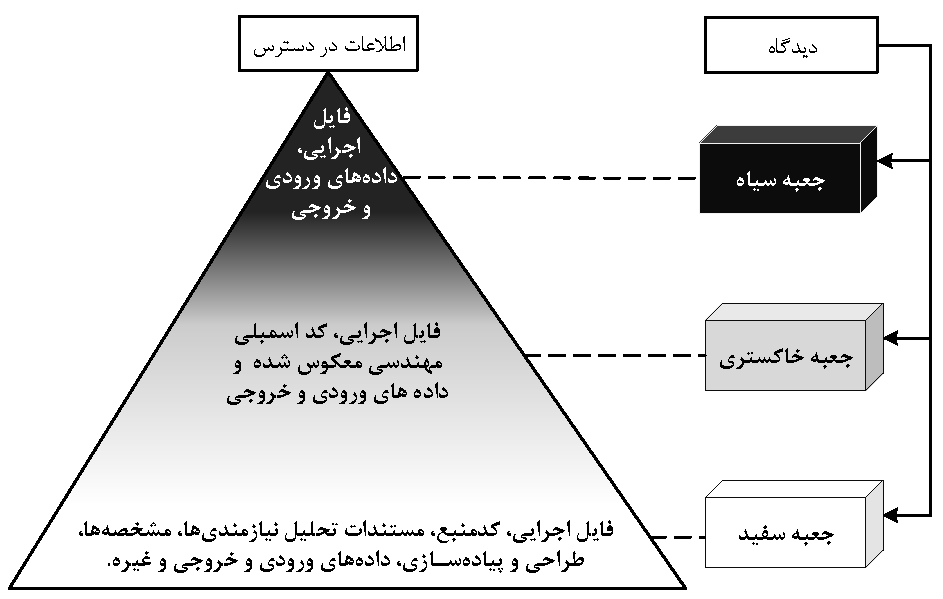
\includegraphics[width=\textwidth, clip=true,  trim= 0 0 0 0]{chapter2/ch2_box_veiw_test_triangle_crop.pdf}
  	%\includegraphics[width=\textwidth]{figs/chapter1/ch1_fuzz_testing_flowchart2.png}
  	\caption[دیدگاه جعبه در آزمون نرم‌افزار]
  	{
  		طرح‌واره‌ای از دیدگاه جعبه بر اساس اطلاعات در دسترس به‌صورت یک مثلث آزمون\cite{ZakeriSeminar2017}.
  	}
  	\label{ch2_box_veiw_test_triangle_crop.pdf}
  \end{figure}
  
  
  همان‌طور که در این طرح‌واره پیداست، در رأس مثلث، هیچ اطلاعی از ساختار داخلی \gls{SUT} در اختیار آزمون‌گر نیست. در واقع با برنامه به مثابه یک جعبه سیاه که ورودی را دریافت و خروجی تولید می‌کند، رفتار می‌شود. این نوع آزمون معمولاً روی برنامه‌هایی که منتشر شده‌اند و توسط افرادی خارج از تیم توسعه و پشتیبانی محصول انجام می‌شود. هدف آن هم بیشتر کشف آسیب‌پذیری‌‌ها و ضعف‌های امنیتی است. در پایین مثلث، دیدگاه جعبه سفید وجود دارد. در اینجا تقریباً تمامی اطلاعات \gls{SUT} در دسترس است. دیدگاه جعبه خاکستری مابین دو دیدگاه قبلی قرار دارد. در این دیدگاه از فنون مهندسی معکوس برای استخراج اطلاعات از \gls{SUT} استفاده می‌شود. هریک از این دیدگاه‌ها مزایا و معایب خاص خود را دارند\cite{Khan2012}. آزمون فازی هم که در ادامه مطرح می‌شود، قابل تقسیم به‌این سه دسته است. آزمون فازی جعبه خاکستری، برای مثال، بسیار ثمربخش بوده است   \cite{DBLP:journals/corr/abs-1711-04596, Zalewsky2013}. روش پیشنهادی در این پایان‌نامه برای تولید داده آزمون، قابل استفاده در هر سه دسته آزمون فازی است. برای ارزیابی روش پیشنهادی در این پایان‌نامه، در \hyperref[ch:5]{فصـل 5}، اما از آزمون جعبه سفید، استفاده کرده‌ایم تا بتوانیم معیارهای پوشش کد و بخش‌های اجرا شده را به‌دقت اندازه‌گیری نماییم. از طرفی \lr{SUT} انتخابی ما متن باز و رایگان بوده و در این حالت کد منبع آن دردسترس است. 
 
     
  \subsection{اندازه‌گیری پوشش کد}\label{sec:instrumenting}
   هدف از مطرح کردن دیدگاه جعبه در بخش \ref{box_view}، اشاره به امکانات لازم برای اندازه‌گیری معیارهای پوشش از جمله پوشش کد بود. در آزمون جعبه سفید که کد منبع برنامه وجود دارد، مشاهده پوشش کد برنامه با اضافه کردن دستوراتی به متن کد به آسانی امکان پذیر است. این عمل را \gls{Instrumenting} کد یا تجهیز برنامه به کد رهگیری می‌نامند\cite{Rathaus:2007:OSF:1536880}. در محیط \lr{GNU/GCC} (زبان‌های \lr{C} و \lr{C++})، برای \gls{Instrumenting} کافی است کد منبع برنامه را همراه با پرچم‌های
   \lr{\texttt{-fprofile-arcs}}
   و
   \lr{\texttt{-ftest-coverage}}
   کامپایل کنیم:\\
   
   
   \begin{LTR}
   	\begin{lstlisting}[language=bash, caption={\rl{ابزارگذاری کد در محیط \lr{GNU/GCC}.}}, label={codesnip2}]
   	~$ gcc -g -fprofile-arcs -ftest-coverage -o test test.c
   	~$ ./test f1 f2
   	~$ gcov test.c
   	~$ more test.c.gcov\end{lstlisting}
   \end{LTR}
سطر اول برنامه \ref{codesnip2} برنامه \lr{test} را با پرچم‌های ذکر شده کامپایل می‌کند. سطر دوم برنامه را با دو آرگومان خط فرمان \texttt{f1} و \texttt{f2} اجرا می‌کند. سطر سوم پوشش کد اجرای اخیر برنامه را محاسبه و فایلی تحت عنوان \texttt{ test.c.gcov} تولید می‌کند. در سطر چهارم این فایل برای مشاهده باز می‌شود. افزون بر این، پرچم‌هایی برای اخذ انواع سطوح پوشش کدی که بحث شد، از جمله پوشش شاخه، وجود دارد \cite{Rathaus:2007:OSF:1536880}. 

  محیط ویژوال استادیو ابزار \lr{vsinstr} را برای ابزارگذاری کد برنامه و \lr{VSPerfMon} را برای اندازه‌گیری پوشش کدِ زبان‌های پشتیبانی شده توسط این محیط، ارائه می‌دهد که البته در حضور کد منبع برنامه قابل استفاده هستند. هنگامی که کد منبع در اختیار نباشد کار اندکی دشوار می‌شود. در این موارد، بایستی از ابزارهای مهندسی معکوس و ابزارگذاری کد باینری استفاده کرد.
 \lr{DynamoRIO}\LTRfootnote{\href{http://www.dynamorio.org/}{http://www.dynamorio.org/}}\cite{Bruening:2004:ETC:1087758}،
 \lr{Pin}\LTRfootnote{\href{https://software.intel.com/en-us/articles/pin-a-dynamic-binary-instrumentation-tool}{https://software.intel.com/en-us/articles/pin-a-dynamic-binary-instrumentation-tool}}\cite{Luk:2005:PBC:1064978.1065034}،
 \lr{PaiMei}\LTRfootnote{\href{https://github.com/OpenRCE/paimei}{https://github.com/OpenRCE/paimei}}\cite{Rathaus:2007:OSF:1536880}
  و 
  \lr{QEMU}\LTRfootnote{\href{https://www.qemu.org/}{https://www.qemu.org/}} \cite{QEMU2018}
 ابزارهایی برای این منظور فراهم کرده‌اند.


  
\section{آزمون فازی}
\gls{FuzzTesting}\cite{Miller:1990:ESR:96267.96279,Miller1995,Forrester:2000:ESR:1267102.1267108,Miller:2006:ESR:1145735.1145743}
همان‌طورکه قبلاً هم گفتیم، فرایند ساده تولید و سپس تزریق یک ورودی ناخواسته (بدشکل شده یا نامتعارف) به \gls{SUT} است. چنان‌چه برنامه بر اثر پردازش این ورودی ناخواسته دچار خرابی شود، حافظه برنامه مورد تحلیل قرار گرفته و خطای احتمالی موجود در کد آشکار می‌گردد. به دلیل اینکه \gls{SUT} هنگام آزمون اجرا می‌شود، آزمون فازی، نوعی آزمون پویا است. چون \gls{SUT} با تعداد ورودی‌های بسیار زیادی مورد آزمون قرار می‌گیرد، آزمون فازی را می‌توان نوعی\gls{StressTesting} هم به‌شمار آورد. فرایند معمول آزمون فازی در ‏شکل
\ref{ch2_fuzz_testing_flowchart_crop.pdf} نشان داده شده است.


%% Need to crop all figures
%% https://pdfresizer.com/
%%
\begin{figure}%[tbh!]%[ht]%[t!]
	\centering
	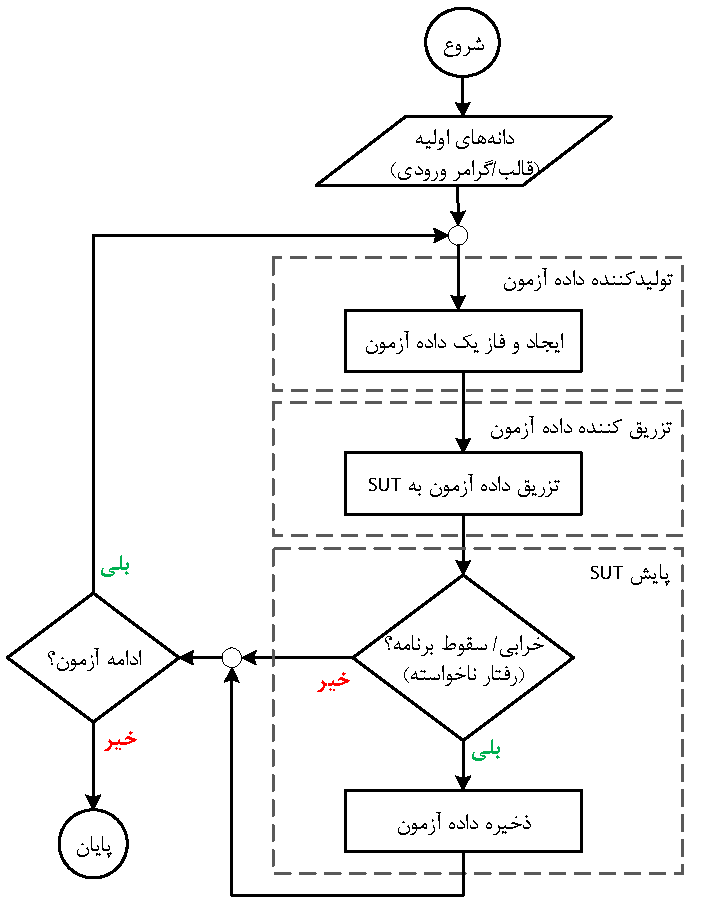
\includegraphics[width=0.9\textwidth, clip=true,  trim= 0 0 0 0]{chapter2/ch2_fuzz_testing_flowchart_crop.pdf}
	%\includegraphics[width=\textwidth]{figs/chapter1/ch1_fuzz_testing_flowchart2.png}
	\caption[روندنمای  فرایند آزمون فازی]
	{
		روندنمای فرایند آزمون فازی در حالت ساده که با اقتباس از مراجع مختلف ترسیم شده است. پیمانه‌های مورد نیاز برای خودکارسازی فرایند با مستطیل خطچین مشخص شده‌اند. شرایط ادامه آزمون می‌تواند بر عهده فرد آزمون‌گر قرار داده شود یا توسط خود فازر تعیین گردد.
	}
	\label{ch2_fuzz_testing_flowchart_crop.pdf}
\end{figure}



\subsection{فازر}\label{sec:fuzzer}
\gls{Fuzzer} ابزاری است که فرایند آزمون فازی را خودکار می‌کند. پیاده‌سازی هریک از \gls{Module}‌های شکل
\ref{ch2_fuzz_testing_flowchart_crop.pdf}
و تجمیع آنها در کنار یکدیگر یک \gls{Fuzzer} را ایجاد می‌کند. تمرکز اصلی در یک \gls{Fuzzer}، نحوه تولید ورودی جدید به عنوان داده آزمون است به‌گونه‌ای که می‌توان آن را وجه تمایز اصلی فازرهای مختلف دانست. روش‌های تولید داده در فازرها قابل تفکیک به دو دسته کلی روش‌های \gls{MutationBased} یا جهش و روش‌های \gls{GenerationBased} 
هستند \cite{Chen2018}.


در روش \gls{MutationBased}، تعداد یک یا بیشتر داده ورودی \gls{Valid} به‌عنوان \gls{InitialSeed} برای تولید داده‌های آزمون بیشتر به‌کار می‌رود.  \gls{InitialSeed} جهش (تغییر ناگهانی) می‌یابد تا داده آزمون دیگری تولید شود. جهش می‌تواند ساده باشد؛ شبیه معکوس کردن یک بیت، جایگزین کردن یک کاراکتر، یا پیچیده‌تر باشد؛ شبیه شناسایی و تکرار ساختارهای مشخص در داده، جایگزینی اعداد صحیح و حقیقی با مقادیر مرزی (بسیار بزرگ یا کوچک) و غیره. ساختن یک فازر مبتنی بر جابه‌جایی و تولید ورودی بد شکل و مخرب با آن، آسان است و نیاز به شناخت قبلی ساختار داده ورودی مورد جهش ندارد. عیب روش مبتنی بر جابه‌جایی اینجاست که این روش وابسته به تنوع ورودی‌های نمونه است. بدون وجود ورودی‌های مختلف با پیچیدگی کافی، این نوع فارز‌ به پوشش کد بالایی دست نمی‌یابد \cite{Kettunen2014}. به عبارت دیگر دانه اولیه در فازر مبتنی بر جابه‌جایی بسیار حائز اهمیت است.
 \lr{AFL}\LTRfootnote{American Fuzzy Lop (\href{http://lcamtuf.coredump.cx/afl/}{http://lcamtuf.coredump.cx/afl/})}\cite{Zalewsky2013}، \lr{FileFuzz}\LTRfootnote{\href{http://www.fuzzing.org/}{http://www.fuzzing.org/}}\cite{Sutton:2007:FBF:1324770}
 و
  \lr{Radamsa}\LTRfootnote{\href{https://gitlab.com/akihe/radamsa}{https://gitlab.com/akihe/radamsa}}\cite{Kettunen2014}
 نمونه‌هایی از فــازرهای مبتنی بر جابه‌جایی هستند.
 
 
 روش مبتنی بر تولید، داده‌های آزمون را به‌صورت کاملاً تصادفی یا از روی یک توصیف صوری مانند گرامر، قالب، یا مدل تولید می‌کند. در حالت دوم، از مشخصه‌های داده ورودی، برای ساخت یک \gls{GenerativeModel} استفاده می‌شود. این روش بیشتر روی قالب‌های داده‌ای که مستنداتی از مشخه‌های آنها در دسترس است، به‌کار می‌رود که در مقایسه با فازرهای مبتنی بر جابه‌جایی، معمولاً به پوشش کد بالاتری دست می‌یابد. با این حال، همان‌طور که در فصل 1 هم اشاره شد، زمان و هزینه زیادی باید صرف شود تا مشخصه‌های یک قالب داده، کامل فهمیده و مدل خوبی از آن تهیه شود؛ زیرا، این کار تمام خودکار نیست \cite{Miller2007} و از طرفی، مستندات ساختار ورودی همواره در دسترس آزمون‌گر، نیستند.
 SPIKEfile\LTRfootnote{\href{http://fuzzing.org/}{http://fuzzing.org/}}\cite{Sutton:2007:FBF:1324770} و
 Peach\LTRfootnote{\href{https://www.peach.tech/}{https://www.peach.tech/}}
 نمونه‌ای از فازرهای مبتنی بر تولید هستند. روش‌های ترکیبی نیز وجود دارد که از ویژگی‌های هر دو روش بیان شده در تولید مورد آزمون کمک می‌گیرد. یک مثال از فازرهای ترکیبی LangFuzz \cite{Holler2012} است.
 
 
 \subsection{معماری فازرها}\label{sec:fuzzers_architechture}
 یک معماری مرجع برای فازرها وجود ندارد؛ ولی می‌توان از روی فرایند ترسیم شده برای آزمون فازی (شکل  \ref{ch2_fuzz_testing_flowchart_crop.pdf})، پیمانه‌های اصلی لازم برای یک فازر را پیشنهاد کرد. پیمانه اول تولید کننده \gls{TestData}است که داده‌های ورودی لازم برای آزمون را تولید می‌کند. دیدیم که روش‌های مختلفی برای تولید داده آزمون وجود دارند. پیمانه دوم تزریق کننده داده آزمون است که وظیفه آن تحویل داده‌های تولید شده توسط تولیدکننده به \gls{SUT} است. هر برنامه واسط مختص به خود را دارد. واسط می‌تواند \gls{CLI}، گرافیکی (\gls{GUI})، پروتکل شبکه یا فایل باشد. هدف این پایان‌نامه برنامه‌هایی هستند که ورودی آنها فایل است. معمولاً داده‌های ورودی به‌شکل فایل (مثل \gls{PDF}) ساختار پیچیده‌تری نسبت به داده‌های \gls{CLI} و پروتکل‌های شبکه دارند و تولید آنها سخت‌تر است. فازری که برای آزمون این برنامه‌ها توسعه داده می‌شود، \gls{FileFormatFuzzer} هم نامیده می‌شود \cite{Sutton:2007:FBF:1324770}.
 
 
 آخرین پیمانه مورد نیاز ابزار یا محیط پایش است که \gls{SUT} را پایش می‌کند تا در صورت بروز خرابی ضمن ذخیره حالت برنامه، محل وقوع خرابی را بتواند با تحلیل حافظه برنامه مشخص کند. البته ابزارهای مستقل زیادی برای این منظور وجود دارند که می‌توان از آنها بهره گرفت. 
 \lr{Application Verifier}\LTRfootnote{\href{https://docs.microsoft.com/en-us/windows-hardware/drivers/debugger/application-verifier}{https://docs.microsoft.com/en-us/windows-hardware/drivers/debugger/application-verifier}}
 \cite{ApplicationVerifier}
 یک ابزار پایشِ قابل استفاده در سیستم عامل ویندوز است. ممکن است فازر، یک بازخورد از ابزار پایش برای تولید داده آزمون بعدی دریافت کند. این بازخورد عموماً حاوی اطلاعات مربوط به پوشش کد اجرای برنامه است. بر این اساس فازرها به دو دسته دارای حلقه بازخورد و بدون حلقه بازخورد تقسیم‌بندی می‌شوند \cite{Chen2018}.
 AFL\cite{Zalewsky2013}
 یک فازر دارای حلقه بازخورد است. در این پایان‌نامه یک فازر ساده قالب فایل بدون حلقه بازخورد ارائه می‌دهیم. تمرکز برروی نحوه تولید داده آزمون به روش \gls{GenerationBased} / گرامر است.
 
 
 
 \subsection{آسیب‌پذیری}
 آزمون فازی می‌تواند برای اهداف مختلفی استفاده شود، اما مهمترین هدف آن تحلیل نرم‌افزار به منظور کشف آسیب‌پذیری‌ها است. یعنی می‌توان آن را نوعی \gls{PenetrationTesting}، \gls{RobustnessTesting} و \gls{SecurityTesting} هم تعریف کرد. تعاریف گوناگونی برای اصطلاح آسیب‌پذیری نرم‌افزار وجود دارد. آسیب‌پذیری را می‌توان اجتماع سه عنــصر دانست: وجود یک خطا در نرم‌افزار، دسترسی مهاجم به خطا و قابلیت مهاجم برای \gls{Exploit} از خطا \cite{Chen2018,InternetSecurityGlossary}. چنانچه پیش از این اشاره شد، خطا، نرم‌افزار را در یک حالت اشکال قرار می‌دهد که منجربه خرابی می‌شود. بعضی خطاها ممکن است تنها منجربه خرابی نرم‌افزار و بروز رفتار ناخواسته (مغایر با مشخصه‌ها) شوند. بنابراین صرف وجود یک خطا در نرم‌افزار آسیب‌پذیری محسوب نمی‌گردد 
 \cite{Sutton:2007:FBF:1324770,Rathaus:2007:OSF:1536880}.
 
 
 انواع مختلفی از خطاها وجود دارند که می‌توانند توسط فازرها کشف شوند؛ به‌ویژه آنهایی که از جنس نقض دسترسی به حافظه هستند. خطاهای فساد حافظه بدون شک رایج‌ترین و مؤثرترین روش بهره‌برداری خرابکارانه از یک سیستم کامپیوتری محلی یا راه دور هستند. اگر حافظه بتواند به روشی خراب شود (یک آدرس بازگشت، یک اشاره‌گر پشته، یک اشاره‌گر تابع و غیره) اغلب اجرا می‌تواند به کد تهیه شده توسط مهاجم هدایت شود. بیشترین آسیب‌پذیری‌هایی که معمولاً توسط محققین حوزه امنیت کشف می‌شوند، مرتبط با \gls{Buffer} (یک ناحیه ثابت از حافظه اصلی در اختیار برنامه) هستند؛ از جمله سرریز میانگیر، سرریز پشته، سرریز عدد صحیح و غیره \cite{Takanen:2008:FSS:1404500}. در آزمون فازی به‌دنبال یافتن چنین خطاهایی از طریق تزریق ورودی بدشکل و خرابی حافظه \gls{SUT} هستیم. مطالعه و طبقه‌بندی کاملی از انواع آسیب‌پذیری‌ها در \cite{ZakeriSeminar2017} انجام شده است.  
 
 
 
 
 %%%%%%%%%%%%%%%%%%%%%%%%%%%%%%%
 %%%  Deep Learning Section  %%%
 %%%%%%%%%%%%%%%%%%%%%%%%%%%%%%%
 
 \section{یادگـیری ژرف}
  \gls{DeepLearning}
مجموعه‌ای از فنون یادگیری ماشینی است که در آن بردار ویژگی‌ها به‌صورت خودکار از داده‌های خام استخراج می‌گردد. ابزار اصلی و غالب در این فنون از یادگیری،  \glspl{NeuralNetwork} هستند. در حالت ساده \glspl{NeuralNetwork} به مسئله یک تابع را نسبت داده و آن را مدل می‌کند. پارامترهای این تابع سپس در فرایند آموزش مدل، تخمین زده می‌شوند. در \gls{DeepLearning} تعداد این پارامترها صدها، هزارها و گاهی میلیون‌ها برابر افزایش می‌یابد که در نتیجه قدرت  \gls{Representation} و حل مسئله مدل، افزایش خواهد یافت. شبکه عصبی در این حالت یک گراف با ژرفای بیش از یک یال، خواهد بود که به آن \gls{DeepNeuralNetwork} هم می‌گویند. شبکه عصبی ژرف بدین ترتیب قادر به استخراج و تمییز جزئی‌ترین ویژگی‌های مسئله و در نتیجه بهبود دقت حاصله، خواهد بود \cite{Goodfellow-et-al-2016}.
 
 
 وجود تعداد بسیاری پارامتر در مدل‌های یادگیری ژرف، سبب می‌شود که آموزش این مدل‌ها از لحاظ محاسباتی سنگین و زمان‌بر باشد. بسیاری از موانع تئوری و عملی آموزش این مدل‌ها به‌تازگی رفع شده‌اند. برای مسائل مختلف، مدل‌های متفاوتی با شبکه‌های عصبی ژرف طراحی و ساخته می‌شوند. \gls{FeedforwardNeuralNetwork} ساده‌ترین نوع است. شبکه عصبی پیچشی (\gls{CNN}) مناسب وظایف بینایی ماشین و شبکه عصبی مکرر (\gls{RNN}) مناسب وظایف پردازش زبان طبیعی (\gls{NLP}) (وظایف مبتنی بر \gls{Sequence}) ایجاد شده‌اند. وجه مشترک همه شبکه‌های نام‌برده، بلوک سازنده آن یعنی \gls{Neuron} است \cite{Jurafsky2017}. 
 
 
 
 \subsection{عصب}
 بلوک محاسباتی پایه در بستر شبکه‌های عصبی، \gls{Neuron} یا \gls{Unit} است. یک عصب تعدادی عدد حقیقی را به‌عنوان ورودی گرفته، محاسباتی روی آنها انجام داده و یک خروجی تولید می‌کند. محاسبه بدین صورت است که عصب جمع وزن‌دار ورودی‌هایی که به آن وارد می‌شوند را به همراه یک مقدار اضافی به عنوان \gls{Bias} حساب می‌کند. سپس برای جلوگیری از محدود شدن فضای توابع قابل تخمین به فضایی خطی، یک تابع غیرخطی، موسوم به \gls{ActivationFunction} (تابع فعّالیت)، روی حاصل جمع اعمال می‌شود. توابع انگیزش متداول عبارتند از \lr{sigmoid} و \lr{tanh}. شکل \ref{ch2_single_neuron_internal_structure_crop.pdf} ساختمان داخلی یک عصب تنها با ورودی‌های $x_1 $، $ x_2 $ و $ x_3 $، متقابلاً وزن‌های $ w_1 $، $ w_2 $ و $ w_3 $ و مقدار بایاس $ b $ را نشان می‌دهد. محاسبات این عصب مطابق رابطه‌های \ref{NeuronActivation} و \ref{NeuronActivation2} است.
 \begin{equation}\label{NeuronActivation}
 z = b+ \sum_iw_ix_i 
 \end{equation}
 \begin{equation}\label{NeuronActivation2}
 y = \sigma(z)
 \end{equation}
 
 
 رابطه \ref{NeuronActivation} را می‌توان به صورت ضرب داخلی بردارهای $ W $ و $ x $ هم نشان داد که نمایش مرسوم‌تری است \cite{Jurafsky2017}:
  \begin{equation}\label{NeuronActivation3}
 z = b+ W.x
 \end{equation} 
 
 
 \begin{figure}%[ht!]%[tbh!]%[ht]%[t!]
 	\centering
 	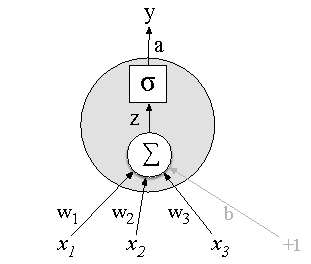
\includegraphics[width=0.5\textwidth, clip=true,  trim= 0 0 0 0]{chapter2/ch2_single_neuron_internal_structure_crop.pdf}
 	%\includegraphics[width=\textwidth]{figs/chapter1/ch1_fuzz_testing_flowchart2.png}
 	\caption[ساختمان داخلی یک عصب]
 	{
 		ساختمان داخلی یک عصب با ورودی‌های $x_1 $، $ x_2 $ و $ x_3 $، به‌ترتیب با وزن‌های $ w_1 $، $ w_2 $ و $ w_3 $، مقدار بایاس $ b $ و خروجی $y$ \cite{Jurafsky2017}.
 	}
 	\label{ch2_single_neuron_internal_structure_crop.pdf}
 	%\ref{ch2_single_neuron_internal_structure_crop.pdf}
 \end{figure}
 
 
 
 \subsection{شبکه عصبی روبه‌جلو}
 شبکه روبه‌جلو را می‌توان با یک گراف جهت‌دار بدون دور (\gls{DAG}) نشان‌ داد. هر گره یک عصب را نشان می‌دهد. گره‌هایی که مسیری به یکدیگر ندارند، یک لایه را تشکیل می‌دهند. ورودی هر لایه، خروجی عصب‌های لایه قبلی است. هر لایه بازنمایی یک \gls{Concept} در قالب یک تابع است و مسئله ترکیبی از این \glspl{Concept} است. یک شبکه با دو لایه تابع 
 $ f(x)=W_2\sigma(W_1 x) $
 را پیاده می‌کند که $ W_1 $ و $ W_2 $  ماتریس پارامترهای تابع و $ \sigma $ تابع انگیزش است.
 $ f(x)=W_3\sigma(W_2\sigma(W_1 x)) $
 معرف یک شبکه سه‌لایه خواهد بود. شکل \ref{ch2_feed_forward_neural_network_crop.pdf} دو گراف محاسباتی با ژرفای 2 و 3 لایه (به ترتیب از چپ به راست) را نشان می‌دهد. لایه‌های میانی را \glspl{HiddenLayer} هم می‌گویند. توجه شود که ورودی اول شبکه یک لایه محاسباتی نیست و بنابراین در شمارش لایه‌ها، شمرده نمی‌شود.
 
 
     
 \begin{figure}[ht!]%[tbh!]%[ht]%[t!]
 	\centering
 	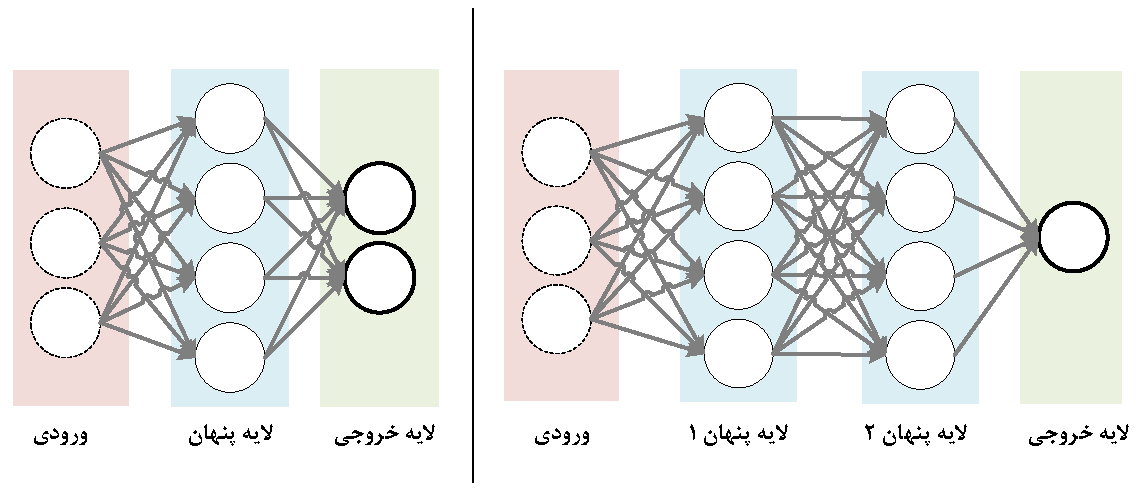
\includegraphics[width=\textwidth, clip=true,  trim= 0 0 0 0]{chapter2/ch2_feed_forward_neural_network_crop.pdf}
 	%\includegraphics[width=\textwidth]{figs/chapter1/ch1_fuzz_testing_flowchart2.png}
 	\caption[گراف محاسباتی شبکه عصبی روبه‌جلو]
 	{
 		گراف محاسباتی برای دو شبکه عصبی روبه‌جلوی فرضی. چپ: یک شبکه عصبی دو لایه (یک لایه پنهان متشکل از چهار عصب و یک لایه خروجی متشکل از دو عصب) به‌همراه سه ورودی. راست: یک شبکه عصبی سه‌لایه (دو لایه پنهان هر کدام متشکل از چهار عصب و یک لایه خروجی متشکل از یک عصب) و به‌همراه سه ورودی. 
 	}
 	\label{ch2_feed_forward_neural_network_crop.pdf}
 	%\ref{ch2_feed_forward_neural_network_crop.pdf}
 \end{figure}
 
 
 \subsection{آموزش شبکه روبه‌جلو}\label{feedforwardtraining}
 هدف از آموزش شبکه، تعیین مقادیر مناسب برای ضرایب و بایاس‌ها و سپس استفاده از شبکه برای انجام \gls{Task} مورد نظر است. داده‌هایی که در فرایند آموزش شبکه استفاده می‌گردد \gls{TrainingSet} نامیده می‌شوند. داده‌هایی که شبکه با آن مورد سنجش قرار می‌گیرد، \gls{TestSet} نامیده می‌شوند و مجموعه سوم از داده‌ها که در طول فرایند آموزش شبکه برای انتخاب بهترین راهکارهای یادگیری به‌کار گرفته می‌شوند، به نام \gls{ValidationSet} شناخته می‌شوند \cite{Goodfellow-et-al-2016}. 
 
 
 شبکه عصبی در یک راهبرد \gls{Supervised} آموزش می‌بیند. در \gls{SupervisedLearning} هر نمونه در مجموعه داده، علاوه بر بردار ویژگی‌ها با یک \gls{Label} همراه است که نقش ناظر را ایفا می‌کند. \gls{Classification} نمونه‌ای از وظایف \gls{SupervisedLearning} است. در این وظیفه برای هر ورودی، کلاس خروجی آن در زمان آموزش مشخص است.
 
 
 در فرایند آموزش ابتدا پارامترهای شبکه مقداردهی اولیه می‌شوند (معمولاً به‌صورت تصادفی). سپس به ازای هر ورودی از مجموعه آموزش، عصب‌های هر لایه خروجی خود را تولید می‌کنند تا زمانی که خروجی نهایی شبکه تولید شود. این مرحله را \gls{ForwardPass} می‌گویند. از آنجایی که خروجی درست برای ورودی مربوطه در زمان آموزش دردسترس است (\gls{SupervisedLearning})؛ اختلاف مقدار محاسبه شده توسط شبکه ($ \hat{y} $) و مقدار واقعی ($ y $)، توسط تابعی موسوم به \gls{ErrorFunction} یا \gls{CostFunction} یا تابع هدف محاسبه می‌شود \cite{Karpathy2016}. توابع مختلفی برای این منظور می‌توان تعریف کرد. 
 تابع \gls{MeanAbsoluteError} (رابطه \ref{MAELossFunction})، تابع \gls{MeanSquaredError} (رابطه \ref{MSELossFunction}) و تابع \gls{CrossEntropyError} (رابطه \ref{CrossEntropyLossFunction}) توابعی هستند که بسته به وظیفه مورد نظر استفاده می‌شوند \cite{Sautermeister2016}.
\begin{equation}\label{MAELossFunction}
	L_{MAE}(\hat{y}, y; W,b)=\frac{1}{n}\sum_{i=1}^{n}|\hat{y_{i}}-y_{i}|
\end{equation}
\begin{equation}\label{MSELossFunction}
L_{MSE}(\hat{y}, y; W,b)=\frac{1}{n}\sum_{i=1}^{n}(\hat{y_{i}}-y_{i})^2
\end{equation}
\begin{equation}\label{CrossEntropyLossFunction}
L_{CE}(\hat{y}, y; W,b)=-\sum_{i=1}^{n}y_i\log{\hat{y_{i}}}
\end{equation}
 
 در روابط \ref{MAELossFunction} تا \ref{CrossEntropyLossFunction}، $ n $ تعداد نمونه‌ها یا تعداد مشاهده‌ها است. در این پایان‌نامه از تابع \gls{CrossEntropyError} استفاده می‌کنیم که برای وظیفه‌های طبقه‌بندی با بیش از دو کلاس مناسب‌ است \cite{Karpathy2016}. وقتی میزان خطا در گذرجلو مشخص شد، هدف تغییر میزان پارامترهای شبکه به‌نحوی است که خطا کمینه شود (رابطه \ref{argminloss}):
 \begin{equation}\label{argminloss}
 	f^{*} = arg \min_{W,b} L(\hat{y}, y; W,b)
 \end{equation}
که $ f^{*} $ تابع یادگیری شده و مقادیر $ W $ و $ b $ پارامترهای شبکه هستند. سایر مقادیر را که در طول این فرایند یادگیری نمی شوند، \gls{Hyperparameter} می‌نامند. از جمله ابر پارامترها می‌توان به تعداد لایه‌ها و تعداد عصب‌ها در هر لایه اشاره کرد، که از آنها برای تعیین اندازه شبکه استفاده می‌‌گردد.
 
 برای کمینه‌سازی خطا، مشتقات جزئی تابع خطا نسبت به هریک از پارامترها در لایه خروجی محاسبه می‌شود (گرادیان) و سپس این روند از طریق روال \gls{Backpropagation} تا ابتدای شبکه پیش‌ می‌رود و مقدار هر پارامتر درسوی کاهش گرادیان با ضریبی موسوم به \gls{LearningRate} بروزرسانی می‌شود. \gls{LearningRate} عدد کوچکی (در مقیاس صدم و هزارم) در نظر گرفته می‌شود که برای همگرایی آهسته و پیوسته شبکه و جلوگیری از واگرا شدن آن لازم است. \gls{LearningRate} یکی دیگر از \gls{Hyperparameter}های مورد نیاز آموزش شبکه‌های ژرف است. الگوریتم \gls{Backpropagation} در واقع یک کاربرد بازگشتی از قاعده مشتق زنجیری در حساب دیفرانسیل است \cite{Karpathy2016}. در اینجا به بیان جزئیات الگوریتم‌های بهینه‌سازی نمی‌پردازیم؛ چارچوب‌های یادگیری ژرف انواع مختلفی از این الگوریتم‌ها را پیاده‌سازی و در اختیار قرار داده‌اند. توضیحات کاملی از این الگوریتم‌ها در  \cite{Goodfellow-et-al-2016} آمده است.
 
 
 \subsubsection{شرایط توقف آموزش}\label{sec:stop_conditions}
 فرایند آموزش شبکه می‌تواند تا بی‌نهایت ادامه داشته باشد. بنابراین بایستی یک قانون برای توقف آن تعریف شود. گزینه‌‌های زیادی وجود دارد که تحت چه شرایطی آموزش را خاتمه دهیم. همچنین ترکیب این شرایط نیز امکان‌پذیر است. برخی از این شرایط عبارتند از \cite{Sautermeister2016}:
 
 \begin{enumerate}
 	\item{
 	هنگامی که تعداد مشخصی \gls{Epoch} طی شود (هر \gls{Epoch} برابر تعداد تکرارهایی است که برای مرور کل مجموعه آموزش لازم است).
 	} 
 	\item{
 	هنگامی که خطای مجموعه ارزیابی (برای تعداد مشخصی \gls{Epoch} متوالی) کاهش پیدا نکند.
 }

\item{
	هنگامی که تغییرات میزان خطا (برای تعداد مشخصی \gls{Epoch} متوالی) کمتر از یک حد آستانه شود.
} 
\item{
	هنگامی که یک زمان مشخص از فرایند آموزش سپری شود.
} 
\end{enumerate} 



 \subsubsection{منظم‌سازی}
مشکل رایجی که هنگام آموزش شبکه عصبی باید جلوگیری شود اثر \gls{Overfitting} است. \gls{Overfitting} یعنی با کاهش خطا روی مجموعه آموزش، خطای مجموعه‌‌های ارزیابی و آزمون به‌طور ناگهانی افزایش ‌یابد \cite{Goodfellow-et-al-2016}. یک دلیل می‌تواند به‌اندازه کافی بزرگ نبودن اندازه مجموعه آموزش باشد. دلیل دیگر می‌تواند پیچیدگی بسیار بالای مدل باشد. پیچیدگی مدل با تعداد پارامترهای  آن مشخص می‌شود. در پیچیدگی بالا ممکن است مدل، \gls{Noise}های موجود در ورودی‌ها را نیز لحاظ کند و متناسب یا برازنده آن شود. در نتیجه هنگام ارزیابی مدل روی داده‌های \gls{TestSet}، خطا بالا می‌رود \cite{Sautermeister2016}. 

راهکارهای مختلفی برای مقابله با مسئله \gls{Overfitting} مدل پیشنهاد شده است. از این راهکارها تحت عنوان فنون \gls{Regularization} یا تنظیم مدل یاد می‌شود. اغلبِ روش‌‌های شناخته شده، پارامترهای دارای مقادیر بالا را که اثرات نوسانی شدیدی دارند، با تابعی جریمه می‌کنند \cite{Karpathy2016}. روش دیگر برای منظم‌سازی 
\lr{Dropout} \cite{JMLR:v15:srivastava14a}
است که بسیار مؤثر و ساده بوده و در مدل‌های یادگیری ژرف معمولاً از آن استفاده می‌شود. در طول آموزش \lr{Dropout} یک عصب را فقط با احتمال $p$ (یک ابر پارامتر) فعال نگه می‌دارد و در غیر این صورت آن را صفر می‌کند. در نتیجه پیچیدگی مدل تنظیم می‌شود.



 
 \subsection{شبکه عصبی مکـرر}
شبکه‌‌های روبه‌جلو در حل مسائلی که ترتیب ورودی در آنها مهم است، مثل ترجمه ماشینی و سایر وظیفه‌های \gls{NLP}، نارسایی دارند. برای مثال در ترجمه ماشینی هر واژه به واژه‌های قبلی خود وابسته است. در این وظیفه‌ها ورودی به‌صورت یک توالی 
$ x = <x^{(1)}, x^{(2)}, x^{(3)}, ..., x^{(n)}> $
است. غالب وظایف حوزه پردازش زبان طبیعی بدین صورت هستند.


شبکه‌های عصبی مکرر
کلاسی از شبکه‌‌های عصبی هستند که به‌صورت یک گراف جهت‌دار دارای دور بیان می‌شوند. به‌عبارت دیگر ورودی هریک از لایه(های) پنهان یا لایه خروجی افزون‌بر خروجی لایه قبل، شامل ورودی‌ای از \gls{TimeStep} قبل به‌صورت بازخورد نیز می‌شود. ‏شکل \ref{ch2_rnn.pdf} یک \gls{RNN} را نشان می‌دهد که در آن لایه پنهان از \glspl{TimeStep} قبلی بازخورد گرفته است. در هر \gls{TimeStep} 
$ t $
 (از
 $ t=1 $ 
 تا 
 $ t=T $)
 یک بردار 
 $ x^{(t)} $
 از توالی ورودی پردازش می‌شود. معادلات گذرجلو شبکه در $ t $ عبارتند از \cite{Goodfellow-et-al-2016}:
 \begin{equation}\label{rnnformula1}
 z^{(t)}=Ux^{(t)}+Wh^{(t-1)}+b
 \end{equation}
 \begin{equation}\label{rnnformula2}
 h^{(t)}=\sigma(z^{(t)})
 \end{equation}
  \begin{equation}\label{rnnformula3}
 y^{(t)} = Vh^{(t)}+c
 \end{equation}
 \begin{equation}\label{rnnformula4}
 \hat{y}^{(t)}=softmax(y^{(t)})
 \end{equation}
 
 
 
 در روابط \ref{rnnformula1} تا \ref{rnnformula4}، $ b $ و $ c $ بایاس و ماتریس‌های  $ U $، $ V $ و $ W $ به‌ترتیب وزن یال‌‌های لایه ورودی به پنهان، پنهان به خروجی و پنهان به پنهان، پارامترهای شبکه هستند. در لایه خروجی به‌جای تابع انگیزش، تابع \gls{Softmax} اعمال می‌شود. این تابع خروجی شبکه را به‌شکل یک توزیع احتمالی معتبر تبدیل می‌نماید و معمولاً در لایه خروجی مدل‌هایی که برای طبقه‌بندی استفاده می‌شوند، قرار می‌گیرد. تابع بیشینه هموار یک بردار $k$تایی از اعداد حقیقی را به عنوان ورودی دریافت نموده و یک بردار $k$تایی از مقادیر حقیقی در بازه  $ [0,1] $ را به عنوان خروجی می‌دهد به‌طوری که جمع مؤلفه‌‌های آن برابر یک خواهد بود (رابطه \ref{softmaxformula}):
 
 \begin{equation}\label{softmaxformula}
 	softmax(x_i) = \frac{e^{x_i}}{\sum_{j=0}^{k}{e^{x_j}}} \quad \textit{\lr{ for i=1 to k}}
 \end{equation}
 
 
 \begin{figure}%[ht!]%[tbh!]%[ht]%[t!]
 	\centering
 	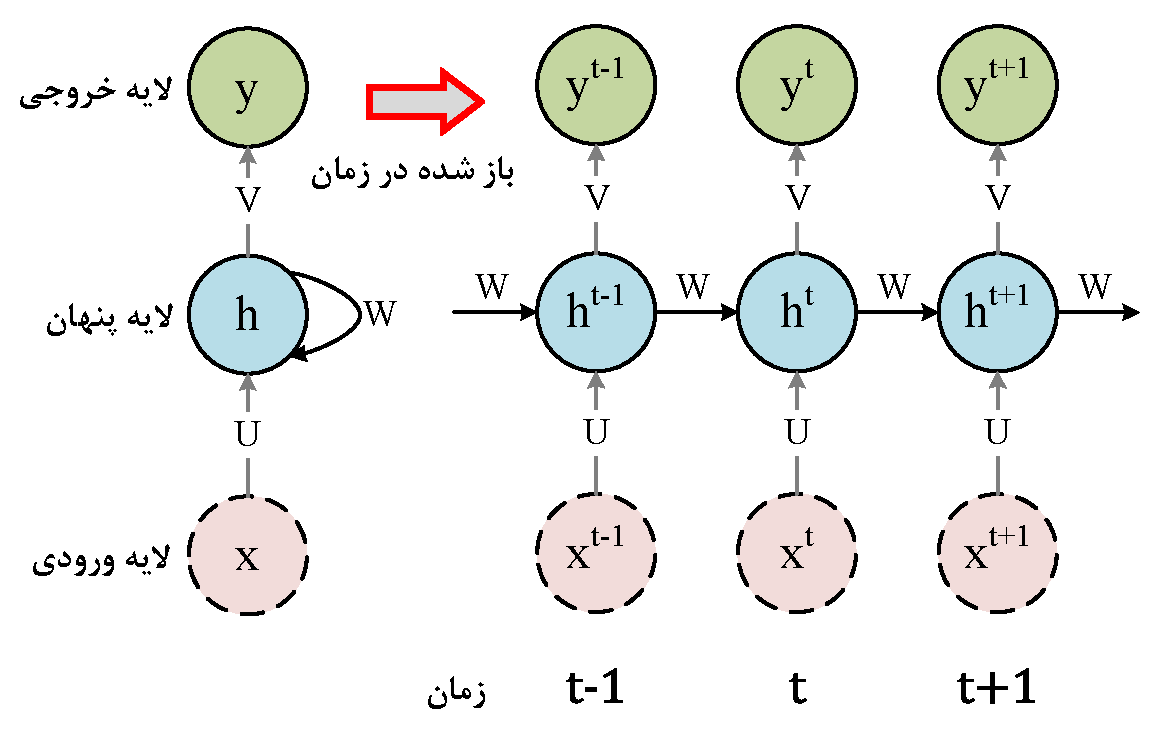
\includegraphics[width=0.8\textwidth, clip=true,  trim= 0 0 0 0]{chapter2/ch2_rnn_crop.pdf}
 	%\includegraphics[width=\textwidth]{figs/chapter1/ch1_fuzz_testing_flowchart2.png}
 	\caption[گراف محاسباتی شبکه عصبی مکرر]
 	{
 		 گراف محاسباتی مربوط به یک شبکه عصبی مکرر با یک لایه پنهان که یک توالی ورودی از مقادیر 
 		 $ x = <x^{(1)}, x^{(2)}, x^{(3)}, ..., x^{(n)}> $
 		 را به یک توالی خروجی از مقادیر 
 		 $ y = <y^{(1)}, y^{(2)}, y^{(3)}, ..., y^{(n)}> $
 		 نگاشت می‌کند. فرض شده است که خروجی $ y $ احتمال‌های نرمال نشده است، بنابراین خروجی نهایی شبکه یعنی $ \hat{y} $ از اعمال تابع بیشینه هموار روی $ y $  حاصل می‌شود. چپ: شبکه عصبی مکرر به‌صورت یال بازگشتی (گراف جهت‌دار دارای دور). راست: همان شبکه به‌صورت باز شده در زمان، به نحوی که هر گره با برچسب مرحله زمانی مشخص شده است \cite{Goodfellow-et-al-2016}.
 	}
 	\label{ch2_rnn.pdf}
 	%\ref{ch2_rnn.pdf}
 \end{figure}
 
 
 
 در ‏شکل \ref{ch2_rnn.pdf}، \gls{RNN} با یک لایه پنهان نشان داده شده است. اما می‌توان \gls{RNN}ژرف با چندین لایه پنهان نیز داشت. همچنین طول توالی‌‌های ورودی و خروجی می‌تواند بسته به مسئله مورد نظر متفاوت باشد. کارپتی\LTRfootnote{A. Karpathy (\href{http://karpathy.github.io/}{http://karpathy.github.io/})}
 	\cite{Karpathy2016}
  \gls{RNN}ها را از منظـر طول توالی ورودی و طول توالی خروجی به چند دسته تقسیم‌بندی کرده است. شکل \ref{ch2_karpathy_rnn_crop.pdf} این دسته‌بندی را نشان می‌دهد.
 
 
 \begin{figure}%[ht!]%[tbh!]%[ht]%[t!]
 	\centering
 	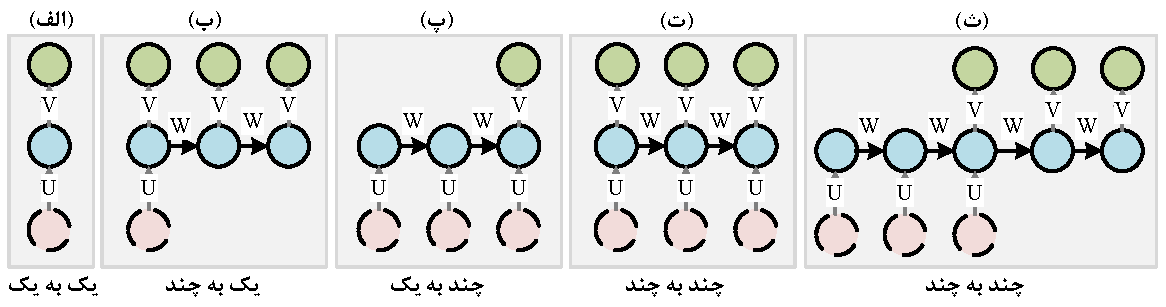
\includegraphics[width=1.0\textwidth, clip=true,  trim= 0 0 0 0]{chapter2/ch2_rnn_karpathy_crop.pdf}
 	%\includegraphics[width=\textwidth]{figs/chapter1/ch1_fuzz_testing_flowchart2.png}
 	\caption[انواع مختلف شبکه عصبی مکرر بر اساس طول توالی ورودی و خروجی]
 	{
 طرح‌واره‌ای از انواع حالت‌های مختلف شبکه عصبی مکرر براساس طول توالی ورودی و طول توالی خروجی. (الف): شبکه عصبی استاندارد، (ب): شبکه یک به چند، (پ): شبکه چند به یک، (ت) و (ث): شبکه‌های چند به چند \cite{Karpathy2016}. 
 	}
 	\label{ch2_karpathy_rnn_crop.pdf}
 	%\ref{ch2_karpathy_rnn_crop.pdf}
 \end{figure}
 
 
 
 \subsubsection{آموزش شبکه عصبی مکرر}
 الگوریتم پس‌انتشار برای آموزش \gls{RNN} هم قابل استفاده است. در واقع \gls{RNN} همان شبکه عصبی روبه‌جلو است که یک بازخورد از وزن‌‌های \gls{TimeStep} قبل دارد. در نتیجه خطا هنوز به‌صورت روی‌به‌عقب از \gls{TimeStep}  $ t $ منتشر می‌شود. بسته به طول توالی ورودی و میزان منابع محاسباتی این انتشار تا \gls{TimeStep}  $ t=1 $ ادامه می‌یابد یا تحت محدودیت تعداد مشخصی \gls{Step} متوقف می‌شود. نسخه‌ای از الگوریتم پس‌انتشار که می‌تواند به‌کل طول توالی ورودی اعمال شود، پس‌انتشار در زمان (\gls{BPTT}) نام دارد. محدودیت منابع محاسباتی ایجاب می‌نماید که طول توالی ورودی مقدار مشخصی قرار داده شود یا پس‌انتشار در تعداد محدودی گام‌زمانی متوقف شود \cite{Goodfellow-et-al-2016}.  
 
 
 \subsubsection{حافظه کوتاه‌مدت بلند}
 \gls{RNN} در حالت استاندارد، برای توالی‌‌های طولانی که وابستگی بین ورودی‌هایی با فاصله زیاد وجود دارد، قادر به حفظ این وابستگی‌ها نیست؛ به‌بیان دیگر گرادیان در دوره‌‌های زمانی بلند مدت تمایل به \gls{Vanishing} یا \gls{Explosion} (زیاد شدن بی‌اندازه) دارد. در حالت ناپدید شدن گرادیان، یادگیری مدل متوقف می‌شود. مدل حافظه کوتاه‌مدت بلند (\gls{LSTM})  برای مقابله با مسئله بالا و افزایش قدرت به‌خاطر‌سپاری   \gls{RNN} ایجاد شده است. هسته این مدل سلول حافظه C است که در آن بر خلاف شبکه مکرر استاندارد که خروجی هر واحد تنها با اعمال یک تابع انگیزش ایجاد می‌شود، خروجی با محاسبات پیچیده‌تری تعیین می‌شود که به‌ویژه هدف آنها منظم‌سازی و حفظ قدرت گرادیان است. ایده اصلی در \gls{LSTM} تخصیص مسیری مجزا علاوه بر یال بازخوردی حالت پنهان، برای جریان حافظه است.
 
 جزئیات عملکرد \gls{LSTM} در \cite{Goodfellow-et-al-2016} توضیح داده شده است. امروزه به‌طور پیشفرض از \gls{LSTM} در پیاده‌سازی \gls{RNN} استفاده می‌شود \cite{DBLP:journals/corr/GreffSKSS15}. البته راه‌کارهای جایگزین دیگری مشابه \gls{LSTM}، نیز مطرح شده‌اند مانند \gls{GRU} \cite{DBLP:journals/corr/ChoMGBSB14}، اما عملکرد آنها بهتر از  \gls{LSTM} نیست. مطالعه جامعی روی \gls{RNN} و انواع آن برای یادگیری توالی‌ها در \cite{DBLP:journals/corr/Lipton15} انجام شده است. کلیه مدل‌های یادگیری ژرف معرفی شده در این پایان‌نامه از \gls{LSTM} در هسته خود استفاده می‌کنند. 
 
 
 
 
 
 
 \section{مدل زبانی}\label{sec:language_model}
 در فصل 
 \ref{chapter1}
 به استفاده از \gls{LM} در روش پیشنهادی خود، اشاره کردیم. 
 \gls{LM} 
 یک مفهوم پایه در \gls{NLP} است که امکان پیش‌بینی نشانه بعدی در یک توالی را فراهم می‌کند. به‌بیان دقیق‌تر \gls{LM} عبارت است از یک توزیع احتمالی روی یک توالی از نشانه‌ها (اغلب واژه‌ها) که احتمال وقوع یک توالی داده شده را مشخص می‌کند. در نتیجه می‌توان بین چندین توالی داده شده برای مثال چند جمله، آن را که محتمل‌تر است، انتخاب کرد. 
 \gls{LM}  
 برای توالی 
 $ x = <x^{(1)}, x^{(2)}, x^{(3)}, ..., x^{(n)}> $
 به‌صورت زیر تعریف می‌شود\cite{Luong2016}:
 \begin{equation}\label{languagemodelformula}
 	p(x) = \prod_{t=1}^{n}p(x^{(t)}|x^{ <t})
 \end{equation} 
 
 
 در رابطه \ref{languagemodelformula} هر جمله منفرد 
 $ p(x^{(t)}|x^{ <t}) $
 احتمال شرطی نشانه 
 $ x^{(t)} $
 به شرط وقوع (ظاهر شدن) $ t $ نشانه قبلی  $ x^{ <t} $ در توالی است که به آن \gls{Context} یا \gls{History} نیز می‌گویند. در عمل محاسبه این احتمال به‌صورت رابطه \ref{languagemodelformula} تقریباً غیر ممکن است؛ زیرا، نیازمند داشتن همه تـوالی‌های ممکن هستیم. مدل‌های سنـتی \lr{n-gram} برای غلبه بر چالش‌های محاسباتی، با استفاده از فرض مارکوف رابطه \ref{languagemodelformula} را به درنظر گرفتن تنها $ n-1 $ نشانه قبلی محدود می‌کنند. اگرچه در بسیاری از مسائل این مدل‌ها به خوبی پاسخ‌گو هستند؛ اما، برای توالی‌های طولانی (بیشتر از 4 یا 5 نشانه) و نیز مشاهده نشده مناسب نیستند. در حالتی که نشانه فعلی پیش‌ از این مشاهده نشده باشد، احتمال صفر به آن نسبت داده می‌شود که سبب صفر شدن احتمال پایانی می‌گردد. برای حل این مشکل، مدل‌های \lr{n-gram} نیازمند اعمال فنون \gls{Smoothing} هستند \cite{Jurafsky2017}. این فنون، راه‌حل‌هایی برای از بین بردن احتمال‌های صفر پیشنهاد می‌دهند. در هر صورت، مدل‌های \lr{n-gram} با محدودیت‌های جدی روبه‌رو هستند.


 
\subsection{مدل زبانی عصبی}
  می‌توان از \gls{RNN} برای ایجاد مدل زبانی استفاده کرد. این مدل‌ها را مدل زبانی عصبی (\gls{NLM}) می‌گویند. استفاده از \gls{RNN} هر دو مشکل اشاره شده در بالا را برطرف می‌کند. یعنی هم امکان پیش‌بینی توالی‌های طولانی‌تر فراهم می‌شود و هم وقوع احتمالات صفر از بین می‌رود \cite{Luong2016}.  شکل \ref{ch2_nlm_persian_crop.pdf} یک معماری از \gls{RNN} برای ساخت مدل زبانی در \gls{NLP} را نشان می‌دهد. چون هدف مدل زبانی پیش‌بینی نشانه بعدی است، توالی $ x $  را در ورودی شبکه قرار داده و خروجی متناظر با آن را همان توالی $ x $ که یک واحد روبه‌جلو شیفت داده شده است، می‌گذارند. این روش آموزش شبکه \lr{Teacher Forcing} می‌گویند \cite{Goodfellow-et-al-2016}.
  
  \begin{figure}%[ht!]%[tbh!]%[ht]%[t!]
  	\centering
  	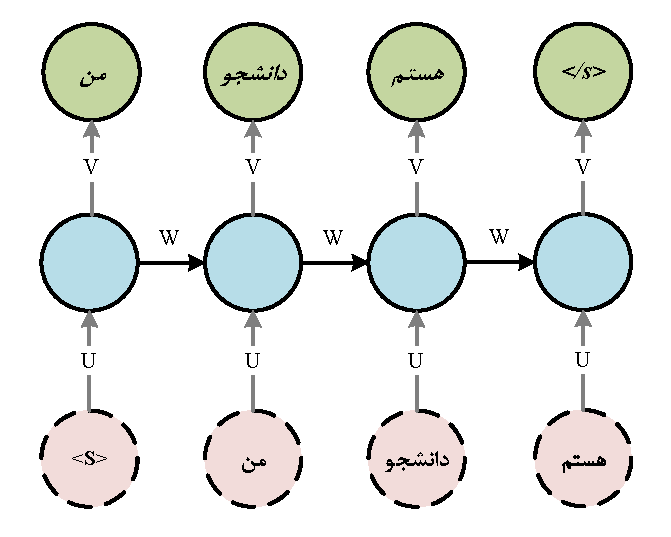
\includegraphics[width=0.7\textwidth, clip=true,  trim= 0 0 0 0]{chapter2/ch2_nlm_persian_crop.pdf}
  	%\includegraphics[width=\textwidth]{figs/chapter1/ch1_fuzz_testing_flowchart2.png}
  	\caption[مدل زبانی عصبی مکرر]
  	{
  		طرح‌واره‌ای از معماری یک مدل زبانی ایجاد شده با استفاده از \gls{RNN}. $ <s> $ نشانه شروع توالی و $ </s> $ نشانه خاتمه توالی در ابتدا و انتهای هر توالی موجود در مجموعه آموزش قرار داده می‌شود. بدین ترتیب، تولید توالی جدید پس از پیش‌بینی نشانه پایان، متوقف می‌گردد \cite{Luong2016}.
  	}
  	\label{ch2_nlm_persian_crop.pdf}
  	%\ref{ch2_nlm_persian_crop.pdf}
  \end{figure}
  
  
  مدل‌های زبانی را \gls{GenerativeModel} نیز می‌نامند؛ زیرا یک توزیع احتمالی روی توالی‌های یک زبان می‌دهند که با نمونه‌‌برداری از آن می‌توان توالی‌های جدید تولید کرد. در \gls{NLP} نشانه‌های هر توالی واژه‌ها هستند، اما می‌توان این مدل را در سطح کاراکتر نیز آموزش داد. ایده اصلی در این پایان‌نامه نیز همین است. هر فایل زبان و قواعد مخصوص به خود را دارد که در مشخصه‌های قالب فایل ذکر شده است. با ایجاد یک مدل زبانی برای این زبان در سطح کاراکتر،  امکان پیش‌بینی نشانه بعدی از روی یک توالی از نشانه‌های داده شده فراهم می‌شود. با نمونه برداری از این مدل زبانی می‌توان داده‌های آزمون جدیدی ایجاد کرد.
 
 \subsection{ارزیابی مدل زبانی}
 چگونه می‌توان میزان خوب بودن یک مدل زبانی را تعیین کرد؟ یک روش برای ارزیابی مدل زبانی، قرار دادن آن در یک وظیفه مشخص و اندازه‌گیری میزان دقت نتایج حاصله است. به این روش‌ \gls{ExtrinsicEvaluation} می‌گویند
 \cite{Jurafsky2017}.
  برای مثال در یک وظیفه تصحیح خودکار غلط‌های املایی، تعداد واژه‌های نادرستی که به‌درستی با واژه‌های صحیح جایگزین شده‌اند را شمارش می‌کنیم و بر تعداد کل واژه‌های غلط تقسیم می‌نماییم. ارزیابی بیرونی، زمان‌بر، پرهزینه و مختص به وظیفه اجرا شده خواهد بود.  روش دیگر استفاده از \gls{IntrinsicEvaluation} است \cite{Jurafsky2017}. معیار \gls{Perplexity} با هدف ارزیابی  درونی مدل زبانی، به‌صورت زیر تعریف می‌شود \cite{mikolov2012statistical}:
  
 \begin{equation}\label{ppl}
 \begin{split}
 	PP_{LM}(x) & = \sqrt[n]{\prod_{i=1}^n(\frac{1}{p(x^{(i)}|<x^{(1)}, ..., x^{(i-1)}>)}} \\
 	& = 2^{-\frac{1}{n}\sum_{i=1}^n\log_{2}{p(x^{(i)}|<x^{(1)}, ..., x^{(i-1)>})}}
 \end{split}
 \end{equation}
در رابطه 
\ref{ppl}،
$ x $
 توالی مورد ارزیابی است. همان‌طور که مشاهده می‌شود \gls{Perplexity} در ارتباط مستقیم با \gls{CrossEntropyError} (رابطه \ref{CrossEntropyLossFunction}) است که میزان اختلاف بین مدل و نمونه‌های مجموعه آزمون را نشان می‌دهد. بنابراین هرچه‌قدر میزان سرگشتگی پایین‌تر باشد، مدل زبانی بهتر است. پایه توان و پایه لـــگاریتم در رابطه \ref{ppl} می‌تواند مقادیری به‌غیر از 2 انتخاب شود. اما در هر حالت هر دو پایه بایستی یکسان باشند تا تساوی اول (بالا) و دوم (پایین) رابطه برقرار گردد. معمولاً از پایه لگاریتم طبیعی در این رابطه استفاده می‌شود 
\cite{DBLP:journals/corr/AbadiABBCCCDDDG16}.

برای درک بهتر نحوه ارزیابی توسط این معیار، توالی 
$ x = <x^{(1)}, x^{(2)}, x^{(3)}, ..., x^{(n)}> $
را در نظر می‌گیریم که متشکل از $ V $ نشانه متفاوت است. $ V $ مجموعه \gls{Vocabulary} زبان است. در غیاب مدل زبانی (بدترین حالت)، تنها می‌توانیم ادعا کنیم که هر نشانه دست‌کم با احتمال 
$ \frac{1}{V} $
در توالی رخ می‌دهد (\gls{BranchingFactor}). بدیهی است که این احتمال برای همه نشانه‌ها یکسان است. برای توالی $ x $ پس از جایگزینی احتمال آن در رابطه  \ref{ppl} داریم:
\begin{equation*}
PP_{LM}(x) = \sqrt[n]{\prod_{i=1}^n(\frac{1}{\frac{1}{V}})} = \sqrt[n]{V^{n}} = V
\end{equation*} 
 بنابراین در بدترین حالت میزان سرگشتگی برابر با اندازه مجموعه \gls{Vocabulary} زبان است. حال چنان‌چه از مدل زبانی استفاده کنیم، احتمال نسبت داده شده به وقوع هر نشانه، نسبت به حالت عدم استفاده از مدل زبانی، افزایش و در نتیجه سرگشتگی کاهش خواهد یافت. در ارزیابی مدل‌های این پایان‌نامه از معیار سرگشتگی استفاده می‌کنیم. 
 
 
 
 
 
 
 \section{خلاصه}
 در این فصل مفاهیم اولیه سه حوزه کلی مطرح در این پایان‌نامه یعنی آزمون نرم‌افزار، آزمون فازی و یادگیری ژرف را بیان کردیم. آزمون نرم‌افزار به‌عنوان یک مسئله تصمیم‌ناپذیر تعریف گردید و معیارهای پوشش برای ارزیابی آن معرفی شدند. آزمون فازی به عنوان یک فن مطرح در آزمون نرم‌افزار، معرفی و از سه دیدگاه مختلف مورد طبقه‌بندی و بحث قرار گرفت: نخست، از دیدگاه اطلاعات در دسترس از \gls{SUT} به سه دسته آزمون جعبه سیاه، جعبه سفید و جعبه خاکستری تقسیم گردید. دوم، از دیدگاه روش‌های تولید داده آزمون به سه دسته مبتنی بر جابه‌جایی، مبتنی بر تولید و نیز ترکیبی تقسیم‌بندی شد. سوم، با توجه به دریافت بازخورد از نتیجه اجرا به دو دسته دارای بازخورد و بدون بازخورد تفکیک گشت. ابزار خودکارسازی آزمون فازی تحت عنوان کلی فازر معرفی و معماری آن تشریح شد.  فازرها با توجه به طبقه‌بندی‌های فوق در بحث آزمون فازی و نیز با توجه به نوع ورودی \gls{SUT} متفاوت هستند. فازرهای قالب فایل مربوط به برنامه‌هایی با ورودی فایل هستند. برای اطلاعات بیشتر در زمینه آزمون نرم‌افزار خواننده را به
  \cite{ammann2016introduction, PaulC.Jorgensen2014} 
 ارجاع می‌دهیم. در زمینه آزمون فازی نیز خواننده را به
 \cite{Chen2018, Mcnally2012, Sutton:2007:FBF:1324770}      
 رجوع می‌دهیم.
 
 در بخش پایانی این فصل، یادگیری ژرف به عنوان زیرشاخه‌ای از یادگیری ماشینی با استفاده از شبکه‌های عصبی مصنوعی، تفهیم شد. شبکه عصبی مورد استفاده در یادگیری ژرف را شبکه عصبی ژرف گویند. \gls{RNN} نوع خاصی از شبکه‌های عصبی ژرف است که برای پردازش وظیفه‌های مبتنی بر توالی مثل مدل زبانی استفاده می‌شود. ساختار یک قالب فایل زبان مختص به خود را دارد و هدف از مطرح کردن اصول اولیه یادگیری ژرف استفاده از مدل‌های این فن، در یادگیری ساختار فایل، جهت تولید داده آزمون جدید است که در فصل 4 به آن خواهیم پرداخت. الگوریتم‌های آموزش شبکه‌های عصبی ژرف ریاضیات گسترده‌ای دارد که به‌طور خلاصه به موارد مهم آن اشاره شد. جهت مطالعه مبسوط این الگوریتم‌ها خواننده را به
 \cite{Goodfellow-et-al-2016}
 ارجاع می‌دهیم. همچنین توضیح کاملی از روش‌های یادگیری توالی با استفاده از \gls{RNN}ها در 
 \cite{DBLP:journals/corr/Lipton15}
 آمده است. در فصل بعد برخی از تازه‌ترین کارهای مرتبط با مفاهیم مطرح شده در این فصل توضیح داده می‌شوند.   
 
 
 
 
 
 
 !
 را در فایل 
 \lr{maintext.tex}،
 غیرفعال%
 \footnote{
     برای غیرفعال کردن یک دستور، کافی است در ابتدای آن، یک علامت
     \%
     بگذارید.
 }
 کنید. 
 در غیر این صورت، ابتدا مطالب دو فصل اول  پردازش شده و سپس مطالب فصل ۳ پردازش می‌شود و این کار باعث طولانی شدن زمان اجرا می‌شود. هر زمان که خروجی کل \پ~ خود را خواستید تمام فصل‌ها را از حالت توضیح خارج کنید.
 
 \subsection{مراجع}
 برای وارد کردن مراجع \پ~ خود، کافی است فایل 
 \lr{\texttt{bibitems/references-all.bib}}
 را باز کرده و مراجع خود را مانند مراجع داخل آن، وارد کنید. سپس از
  \lr{bibtex} 
 برای تولید مراجع با قالب مناسب استفاده کنید.  
 
 \subsection{واژه‌نامه فارسی به انگلیسی و برعکس}
 برای وارد کردن واژه‌نامه فارسی به انگلیسی و برعکس، در این قالب از بسته
 \lr{glossaries}
 استفاده شده است. راهنمای این بسته را می‌توانید به راحتی و با یک جستجوی ساده در اینترنت پیدا کنید.
 
 \subsection{نمایه}
 در استاندارد قالب پایان‌نامه دانشگاه علم و صنعت نمایه وجود ندارد و نیازی به آن نیست با این حال
 برای ایجاد نمایه، این قالب از 
 \lr{xindy}
 استفاده می‌کند.
 
 \section{پرسش‌های متداول}
نسخه عمومی قالب نگارش پایان‌نامه 
\gls{MOST}
روی نشانی 
\href{https://m-zakeri.github.io/ZMOST}{\lr{https://m-zakeri.github.io/ZMOST}}
قرار دارد که با انتشار بسته‌های جدید 
\LaTeX،
در صورت مغایرت و عدم اجرای کدهای فعلی، این قالب بروزرسانی می‌شود. 
بنابراین برای دریافت بروزترین نسخه این قالب، به نشانی فوق مراجعه کنید.
%%
 همچنین برای پرسیدن سؤال‌های خود موقع حروف‌چینی با زی‌پرشین،  می‌توانید به
 \href{http://forum.parsilatex.com}{تالار گفتگوی پارسی‌لاتک}%
 \LTRfootnote{http://forum.parsilatex.com}
 مراجعه کنید. 
 
\section{ساختار پروژه،  پایان‌نامه یا رساله}
 فصل مقدمه به‌طور کلی دارای بخش‌های شرح مسأله، انگيزه‌های پژوهش، مفروضات پژوهش، اهداف پژوهش و ساختار پايان‌نامه است. فصل‌های بعدی به ترتیب تحت عنوان ادبیات موضوع، روش‌ پشنهادی، ارزیابی و نتیجه‌گیری هستند.
 
 %%%%%%
 %% پایان فصل اول
 %%%%%%
